\documentclass[a4paper, 12pt, twoside, openright, table]{book}
\usepackage{geometry}
\usepackage{amsmath}
\usepackage[labelfont=bf]{caption}
\usepackage{subcaption,booktabs}
\usepackage[ruled,noline]{algorithm2e}
\usepackage[printonlyused,withpage]{acronym}
\usepackage[sorting=none, style=numeric, backend=biber, natbib]{biblatex}

\usepackage{graphicx}
\usepackage{hyperref}
\usepackage{cleveref}
\usepackage{setspace}
\usepackage{fancyhdr}
\usepackage{pdfpages}

% Packages added to template
\usepackage{changepage}

% Changed variables
\setcounter{secnumdepth}{3} % how many sectioning levels to assign numbers to
\setcounter{tocdepth}{3}    % how many sectioning levels to show in ToC

% useful to make todos
\usepackage{todonotes}

% you can set the font to calibri, or opensans which closely resembles calibri
\usepackage{fontspec}
% \setmainfont{calibri}
\setmainfont{opensans}

\bibliography{references}

\title{Thesis}
\author{author}
\date{Current Year}

% Turn on the style
\pagestyle{fancy}
% patch chapter style
\usepackage{etoolbox}
\patchcmd{\chapter}{\thispagestyle{plain}}{\thispagestyle{fancy}}{}{}

%\fancyhf{}
\fancyhead[L]{}
\fancyhead[R]{\leftmark}
% Set the right side of the footer to be the page number
\fancyfoot{}
\fancyfoot[R]{\thepage}

\geometry{bottom=2.5cm, top=2.5cm, left=2.5cm, right=2.5cm}
\setstretch{1.5}
\setlength{\parindent}{0pt}
\setlength{\parskip}{6pt}
\setlength{\headheight}{15pt}

\begin{document}
\frontmatter
% plug your own cover page here
%
\includepdf[pages=-]{Cover.pdf}
% some empty pages
%\newpage\null\thispagestyle{empty}
%\newpage\null\thispagestyle{empty}
%\newpage\null\thispagestyle{empty}
%\chapter*{Preface}
\markboth{PREFACE}{} % force the marker to not show "CHAPTER 0. PREFACE"
\thispagestyle{empty} % if desired we can skip the chapter markers entirely on this page
This is the preface to this thesis.



\newpage\null\thispagestyle{empty} % empty page

\tableofcontents
\listoffigures
\listoftables
\chapter*{List of Abbreviations and Symbols}
\begin{acronym}[ABC]\itemsep8.0pt
  \acro{MS}{Mass Spectrometry}
  \acro{MS/MS}{Tandem Mass Spectrometry}

  \acro{SMILES}{Simplified Molecular Input Line Entry System}
  \acro{SELFIES}{SELF-referencIng Embedded Strings}

  \acro{MCES}{Maximum Common Edge Subgraph}

  \acro{SVM}{Support Vector Machine}
  \acro{GUI}{Graphical User Interface}
  \acro{MLP}{MultiLayer Perceptron}
  \acro{VAE}{Variational Auto Encoder}
  \acro{RNN}{Recurrent Neural Network}
  \acro{GRU}{Gated Recurrent Unit}
  \acro{CNN}{Convolutional Neural Network}

  \acro{BPE}{Byte-Pair Encoding}
  
  
  
  
\end{acronym}


\mainmatter
% \input{Abstract}
\chapter{Background}
\label{chap:background}

\section{Tandem Mass Spectrometry}
\label{sec:tandemMS}

\ac{MS} is a method for extracting the composition of a compound using its molecular weight \cite{broad_mass_spectrometry}. It measures the mass-to-charge ratio (m/z) of its ions to provide a spectral view of the compound. Due to its high precision and sensitivity, even the smallest molecules can be analyzed using Mass Spectrometry. Nowadays, Mass Spectrometers can analyze a sample within a few seconds with very high accuracy. This is the reason why it is the go-to method for analyzing unknown compounds \cite{scripps_mass_spectrometry}.

\subsection{Mass Spectrometry}

The basic MS process consists of 3 steps: ionization, mass analysis, detection \cite{broad_mass_spectrometry, garg2024mass}.
Firstly, the sample is ionized. This converts the molecules into charged ions and enables the manipulation by electric and magnetic fields. A common approach is electron ionization (EI). In this method, an electron beam is used to bombard the analyte molecule and knock an electron off, causing the molecule to split into charged ions and fragments according to their molecular structure \cite{scottElectronIonization}. This fragmentation is reproducible which makes the identification of a compound possible.
By using an electric or magnetic field, the ions are then separated based on their mass-to-charge ratio. One such method is using an ion trap, it uses an electric field to capture ions in a small space, holding them in stable orbits \cite{garg2024mass, chong2018clinical}. By gradually adjusting the field, ions are released sequentially by mass-to-charge ratio toward the detector. This allows for highly sensitive separation of the charged ions. The strength of the electric field when a specific ion is released from the tap determines its mass-to-charge ratio.
A detector will then quantify the separated ions \cite{garg2024mass}. These ions can be detected by using an electron multiplier. This device will amplify the signal strength of an incoming ion. When an ion strikes the electron multiplier's surface, it releases secondary electrons. These electrons are accelerated toward a series of dynodes (electrodes), each releasing more electrons upon impact. This cascade effect creates a large, amplified pulse of electrons from a single ion strike. The resulting electrical pulse is proportional to the number of ions, enabling the mass spectrometer to measure ion abundance (intensity) for each m/z value in the mass spectrum.

An example spectrum output from a mass spectrometer is shown as a histogram in Figure \ref{fig:mass_spectrum_example}.

\begin{figure}[h]
    \centering
    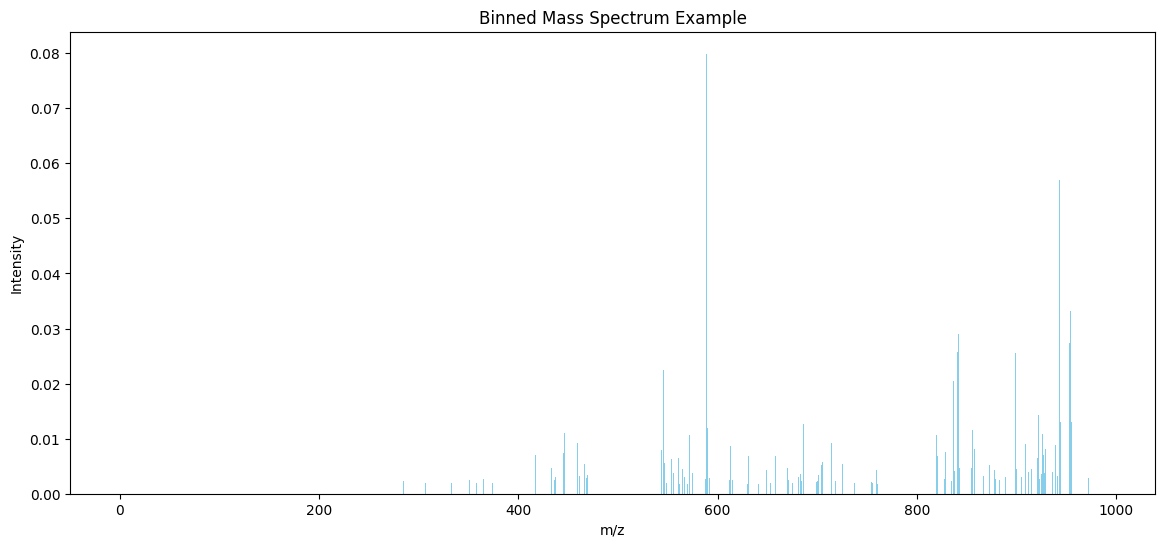
\includegraphics[width=\linewidth]{figures/background/mass_spectrum_example.png}
    \caption{A Mass Spectrum from GNPS, the peaks are binned using a histogram}
    \label{fig:mass_spectrum_example}
\end{figure}

\subsection{\acf{MS/MS}}

To determine the exact chemical structures of an input sample containing unknown molecules using mass spectrometry can be quite hard. Especially when the input sample contains a lot of different large molecules, the output from a single Mass Spectrometry analysis will describe an m/z spectrum of a mixture of ions. These different ions could have similar m/z values causing them to be inseparable. To distinguish them we can fragment ions with the same m/z range from the mixture using another round of Mass Spectrometry. This will fragment the ions further which allows them to be distinguished. This is in essence the goal of Tandem Mass Spectrometry (\acs{MS/MS} or MS$^2$). After ionization, it does multiple rounds of Mass Spectrometry (each with a separation step in between) before the detection step to increase the precision of the analysis \cite{antoniewicz2013tandem, nationalmaglabtand}. This way we can fragment and distinguish ions with similar m/z values.

In the separation step precursor ions are selected. These are ions that have overlapping m/z values that we want to fragment further. To achieve this, an isolation window is chosen with a certain m/z width \cite{defossez2023eight}. This window is used to slide over the spectrum generated by the first round of mass spectrometry to find these precursor ions. This selection is done either algorithmically or hard-coded. These precursor ions are then fragmented using collision-induced dissociation, ion-molecule reaction, or photodissociation. For example: Collision-induced dissociation uses the precusor ions in a gas stage to accelerate them towards neutral molecules \cite{wells2005collision}. The collision causes bonds within the ions to break, which fragments these precursor ions. These fragments can then be detected in the same way as the original mass spectrometry detector. Collision-induced dissociation can cause the molecular structure of an ion fragment to reform because a certain bond was broken, which will be detected as the wrong structure by the detector. Luckily this is mostly not the case \cite{molina2008comprehensive}.

The amount of fragmentation steps can be chosen arbitrarily,
depending on known knowledge about the input molecules or precision needed for downstream analysis.
Mass Spectrometry without fragmentation, where just the separation and mass analysis steps are performed is abbreviated as MS$^1$,
tandem mass spectrometry with one or more rounds of fragmentation, each followed by a separation and mass analysis step, is often abbreviated as MS/MS or MS$^x$ with $x$ denoting the amount of mass analysis steps (= number of fragmentation rounds - 1).

\section{Molecular Representations}
\label{sec:molrepr}

This section discusses different molecular representations and their structures. Representations that are not frequently used in the molecular structure predicting domain are left out. Table \ref{tab:molecularreps} gives an overview of the molecular representations discussed in the following subsections.

%\begin{table}[h]
%    \centering
%	\setlength{\tabcolsep}{20pt}
%    \renewcommand{\arraystretch}{1.5}
%	\caption{
%		Different representations for the molecule Benzene. The Fingerprint representation shows only the first 40 bits for illustrational purposes, followed by three dots to indicate the truncation.
%	}
%	\begin{tabular}{ll}
%    		\toprule
%                    \textbf{Representation} & \textbf{Example} \\
%            \midrule
%    		      Chemical Formula & C$_6$H$_6$\\
%                    (Morgan) Fingerprint & 0000000000000000000000000000000000000010...\\
%                    InchI & InChI=1S/C6H6/c1-2-4-6-5-3-1/h1-6H\\
%                    InchIKey & UHOVQNZJYSORNB-UHFFFAOYSA-N\\
%                    SMILES & c1ccccc1\\
%                    DeepSMILES & cccccc6\\
%                    SELFIES & [C][=C][C][=C][C][=C][Ring1][=Branch1]\\
%    		\midrule
%    	\end{tabular}
%	\label{tab:molecularreps}
%\end{table}
\begin{table}[h]
    \centering
	\setlength{\tabcolsep}{20pt}
    \renewcommand{\arraystretch}{1.5}
	\caption{
		Different representations for the molecule Toluene (Methylbenzene). The Fingerprint representation shows only the first 40 bits for illustrational purposes, followed by three dots to indicate the truncation.
	}
    \resizebox{1.00\linewidth}{!}{
	\begin{tabular}{ll}
    		\toprule
                    \textbf{Representation} & \textbf{Example} \\
            \midrule
    		      Empirical Formula & C$_6$H$_5$CH$_3$\\
                    (Morgan) Fingerprint & 0000000000000000000000000000000000000000...\\
                    InchI & InChI=1S/C7H8/c1-7-5-3-2-4-6-7/h2-6H,1H3\\
                    InchIKey & YXFVVABEGXRONW-UHFFFAOYSA-N\\
                    SMILES & Cc1ccccc1\\
                    DeepSMILES & Ccccccc6\\
                    SELFIES & [C][C][=C][C][=C][C][=C][Ring1][=Branch1]\\
    		\midrule
    \end{tabular}
    }
	\label{tab:molecularreps}
\end{table}

\subsection{Empirical Formula}

The simplest and most well-known representation is the empirical formula. It is a textual representation that numbers the abundance of each element relative to each other. The empirical chemical formula does not describe any structural information and is therefore very unsuitable for describing specific molecular structures \cite{hartshorn2015brief}.

\subsection{Fingerprints}

To encode the chemical structure of a molecule, we could look at certain properties of the molecule instead of encoding the exact structure itself. This is in essence the purpose of molecular fingerprints. They represent properties of a molecule as a bitvector of a certain size which can be fixed or variable. Each bit then encodes the presence or absence of a certain property \cite{kuwahara2021analysis}. The properties that are encoded can vary. These are mostly human-curated specifically for a desired domain.

A few examples of different molecular fingerprints \cite{wigh2022review, kuwahara2021analysis, pharmacorefingerprints}:
\begin{description}
   \item[Structural / Topological fingerprints (e.g. MACCS Keys)]{Each bit represents the presence/absence of a certain molecular fragment. These are mostly used to measure molecular similarity.}
   \item[Circular/Radial fingerprints (e.g. Morgan Fingerprints (used in RDkit))]{These encode atom-centered neighborhoods iteratively. They capture local structural information but do not capture information on explicit connectivity.}
   \item[Pharmacophore fingerprints]{Encode chemical features such as structural properties related to binding.} 
   \item[Machine-learning-based / Embedding fingerprints]{Non-human curated bitvectors which are often a rounded output of an embedding layer from a neural network.}
\end{description}

These fingerprints provide a representation of a chemical structure that can explicitly store a lot of information about the properties of the molecule.
These bitvectors can be used very efficiently in well-established comparison algorithms which makes them very popular in certain machine learning applications that focus only on the properties that are encoded in the molecular fingerprint.
Their main drawback is the way they are encoded.
Because the molecular structure itself is not encoded as a whole, even with structural fingerprints, it is very hard to extract the exact molecular structure because some structural information is lost \cite{kretschmer2023small}.
Different chemical structures can also encode to the same bitvector, because they share the same properties, which can cause confusion.
For these reasons, this molecular representation may not be desirable for describing a molecular structure \cite{dablander2024sort}.

\subsection{InChI}

The International Chemical Identifier (InChI) is a standardized textual representation of a molecular structure developed by IUPAC \cite{heller2015inchi}. InChI has a bijective relation with all molecular structures, which allows each structure to be uniquely represented to prevent ambiguity. It was originally developed (and is still mostly used) for search algorithms to distinguish between different representations of the same molecule. An InChI consists of layered information:
\begin{description}
    \item[Main Layer]Defines core molecular connectivity and hydrogen positions.
    \item[Charge Layer]Captures formal charge states.
    \item[FixedH layer]Allows to distinguish tautomers by their mobile H atoms.
    \item[Stereochemistry Layer]Encodes chiral centers and double-bond configurations.
    \item[Isotopic Layer]Represents isotopic variations.
    \item[Reconnected layer]Metal-containing compounds are split to prevent ambiguity, the original metal bonding scheme is stored here.
\end{description}

Each Identifier starts with "InchI=", followed by each layer separated by a forward slash character.
Not all layers have to be present to describe a valid InChI,
redundant or non-relevant information can be omitted if the base relation of InchI still holds.
This layered textual structure allows the format to be somewhat human-readable.

\subsubsection{InchIKey}

A main drawback of InchI is its length: for big molecular structures it can be very large.
Therefore, to further improve search methods, the InchI can be hashed to drastically reduce its size.
This is exactly what InchIKey achieves.
It is a 27-character compacted representation calculated by combining blocks of SHA256 hashes converted to base26.
These blocks are calculated by hashing the different layers from the InchI string.
The first block, consisting of 14 letters, encodes the core molecular constitution using the main layer.
The second block, with a length of 10 letters, is created by using 8 letters from the hashed remaining layers and 2 letters to denote the InchI type (S for standard N for non-standard) and version (A for version 1).
The last block containing one letter is used to describe in which protonation state the molecule is, with N being neutral.
These three blocks are separated by a hyphen character.

Because InchIKey is hashed, in theory it loses the bijective relation to the chemical structures, as hash collisions (2 InchI mapping to the same InchIKey) are possible.
\textcite{pletnev2012inchikey} have proven, however, that this probability is close to the theoretical expectation which is almost negligible.

While InchI's can be used to reconstruct an exact molecular structure, the one-way encoding using hashing prevents this with InchIKeys. They are only useful for database lookups as the InchIKey itself does not allow any structural information to be extracted. 

\subsection{SMILES}

A \ac{SMILES} string provides a linear textual representation of a molecular structure using ASCII characters.
It was developed to mimic the structure of natural language with its linear string of symbols, while also maximizing its simplicity \cite{weininger1988smiles}. The SMILES generation rules are kept relatively simple while still holding the desired requirements for a chemical notation language. It balances the human-readability with optimization for computer efficiency, striving to be human- and machine-friendly.

SMILES describe a molecular structure as a two-dimensional graph. It encodes the connectivity between atoms.
The SMILES generation rules are as follows:

\begin{itemize}
    \item Atoms are depicted by their atomic symbols in square brackets (except for some organic elements) with the second letter being lowercase. (e.g. [Fe])
    Attached hydrogens (the symbol H with an optional digit following) and formal charges (+ or - with an optional digit following) should also be denoted inside the square brackets.
    \item Bonds are represented by: - for single bonds, = for double bonds and \# for triple bonds. Single bond characters are usually ignored.
    \item Branches are depicted by encapsulation with parentheses.
    \item Cycles are split and represented in any order starting and ending with the same single digit denoting the start and end of the cycle.
    \item Disconnected structures are represented independently with a period used for separation.
    \item Aromatic ring structures are depicted by using lower case letters.
\end{itemize}

These generation rules are still flexible, which allows for multiple SMILES to be "synonyms" of each other.

Because SMILES only represent two-dimensional graphs and only capture the connectivity between atoms, 
they generally lack explicit three-dimensional information, such as the precise spatial orientation, conformational flexibility, and subtle stereochemical details (unless additional annotations are included). Without these extra annotations, multiple chemical structures could map to the same SMILES string, standardization is thus needed to distinguish similar molecular structures.\cite{heller2015inchi}.   

\subsubsection{DeepSMILES}

Because SMILES strives to mimic natural language, the recent breakthroughs in natural language processing using auto-regressive neural networks proved its utility for chemical structure generation.
Its biggest drawback however is that the representation allows for syntactical errors by either (1) unbalanced parentheses and (2) unbalanced ring depictions \cite{o2018deepsmiles}. DeepSMILES \cite{o2018deepsmiles} addresses these issues.
It is a chemical representation built on the same fundamentals as SMILES, with the exception of these two main issues.
In DeepSMILES, ring structures only have a digit at the end to denote the ring size, which implicitly encodes the starting position.
The unbalanced parentheses problem is solved by only using closing parentheses.
The closing parentheses are then repeated, with the amount being equal to the branch length.
With these changes, DeepSMILES can be converted easily to SMILES without any loss of data.

These optimizations for SMILES strings make sure that any string sampled with random (SMILES) characters (except for the opening bracket),
depicts a valid DeepSMILES string,
which is an important feature in autoregressive generation. However it does not address the problem that some strings may violate basic chemistry rules, such as the maximum number of valence bonds between atoms \cite{krenn2020self}.

\subsection{SELFIES}

Another textual molecular representation that strives to have the same benefits as SMILES without the possible syntactical errors is \ac{SELFIES} \cite{krenn2020self}.
Unlike DeepSMILES, they also address the chemical validity of strings. This is achieved by using a context free grammar~\cite{lo2023recent}. A SELFIES string is a combination of tokens. These tokens are restricted by a constraint function to be chemically viable.
This is the key aspect that allow SELFIES to be robust. There are four different kind of tokens:

\begin{description}
    \item[Atom Token] Following the notation of \textcite{lo2023recent}, an atom token has the form:
    \[[\beta\alpha_{iso}\alpha_{elem}\alpha_{chiral}\alpha_{H}\alpha_{\pm}]\]
    where:
    \begin{align*} 
    \beta &\in  \{\varepsilon, = , \#,/, \textbackslash\} \\ 
    \alpha_{iso} &\in  \{\varepsilon,1,2,3,...\} \\
    \alpha_{elem} &\in  \{element\ symbols\} \\ 
    \alpha_{chiral} &\in  \{\varepsilon, @, @@\} \\
    \alpha_{H} &\in  \{\varepsilon,H0,H1,...,H9\} \\
    \alpha_{\pm} &\in  \{\varepsilon,+1,-1,+2,-2,+3,...\}
    \end{align*}
    Beta describes a SMILES-like bond, the alphas describe isotope number, atomic number, chirality, number of attached hydrogens and charge, respectively \cite{lo2023recent}. A lot of information is described with one token, whereas in SMILES there would be a lot of different symbols used.
    
    \item[Branch Token] Following the notation of \textcite{lo2023recent}, a branch token has the form:
    \[[\beta Branch\ \ell]\]
    where:
    \begin{align*} 
    \beta &\in  \{\varepsilon, = , \#\} \\ 
    \ell &\in \{1, 2, 3\}
    \end{align*}
    Again Beta is a SMILES-like bond. A branch token is only put at the end of a branch (similar to DeepSMILES) with the next $\ell$ tokens describing the length of the branch by using predefined tokens to represent certain values. When there are no next tokens, 0 is used.

    \item[Ring Token] Following the notation of \textcite{lo2023recent}, a ring token has one of 2 forms:
    \begin{align*} 
    &[\beta Ring\ \ell] \\ 
    &[\beta_1\beta_2 Ring\ \ell]
    \end{align*} where: \begin{align*} 
    \beta &\in  \{\varepsilon, = , \#\} \\
    \ell &\in \{1, 2, 3\} \\
    \beta_1,\beta_2 &\in \{-, /, \textbackslash\} \\
    \beta_1 = -& \Rightarrow \beta_2 \neq - \\
    \beta_2 = -& \Rightarrow \beta_1 \neq -
    \end{align*}
    Similar to branch tokens, ring tokens are put at the end of a ring enclosure. The size of the ring is calculated in the same way as the length of the branch for branch tokens.

    \item[Miscellaneous Tokens] Miscellaneous symbols are required for SMILES to be easily translatable to SELFIES. An example of a miscellaneous token is the dot symbol. Just as in SMILES it represents a disconnected structure.
    
\end{description}

Because these tokens encode so much information that is stored by multiple symbols in SMILES, by only using a combination of valid tokens, SELFIES strings are completely robust. This means that it always encodes a valid molecular structure while also being able to represent every possible molecule \cite{lo2023recent}. If we would randomly sample from a complete set of tokens, which can be constructed by exhausting the constraint function defined in SELFIES, the result would always map to a valid molecular structure. This is a key aspect which proves its usefulness in the autoregressive generation of SELFIES.

\section{Evaluation Metrics}
\label{sec:evalmetrics}

Quantifying the similarity of molecular representations is crucial for evaluating machine learning models that try to predict these representations. The similarity metric should describe how similar the actual molecular structures of two representations are. The most naive similarity metrics often only describe how similar the representations are to each other without taking the underlying chemical structure into account. This, however, will hinder generalization for the overall molecular structure prediction problem. More advanced metrics are required.

A distinction also needs to be made between structural similarity and property similarity. Property similarity is often the preferred metric in biological settings that are more interested in the properties of the molecules \cite{safizadeh2021improving}. Because this thesis is about predicting molecular structures, only structural similarity metrics are discussed.

\subsection{Tanimoto Similarity}
\label{sec:tan_sim}

The molecular structure can't be directly derived from fingerprints because they don't store complex structural information \cite{kretschmer2023small}. This is a problem for calculating the similarity of the underlying molecular structure of two fingerprints, as we can't construct molecular graphs to calculate an exact structural similarity metric. We have to resort to similarity metrics on fingerprints themselves that would estimate the structural similarity.

Molecular fingerprints are bitvector representations. A naive way to compare two bitvectors would be to calculate the sum of the logical 'and' operation divided by the length of the bitvector, in essence counting the number of bits that are the same. This would only work if the value of each bit has no correlation with any other bit and each bit in the bitvector has an equal occurrence probability. This is not true for molecular fingerprints. They are known to be very sparse and have a non-uniform distribution. For example: Figure \ref{fig:bit_frequency_fingerprints} shows the activation frequency per bit position for a typical fingerprint. It is clear that these are not uniformly distributed with some bits having a very high activation frequency (above 70\%) and a few bits not even being active once. It is clear that the activation frequency of most bits is very low, causing the fingerprints to be sparse.

\begin{figure}[h]
    \centering
    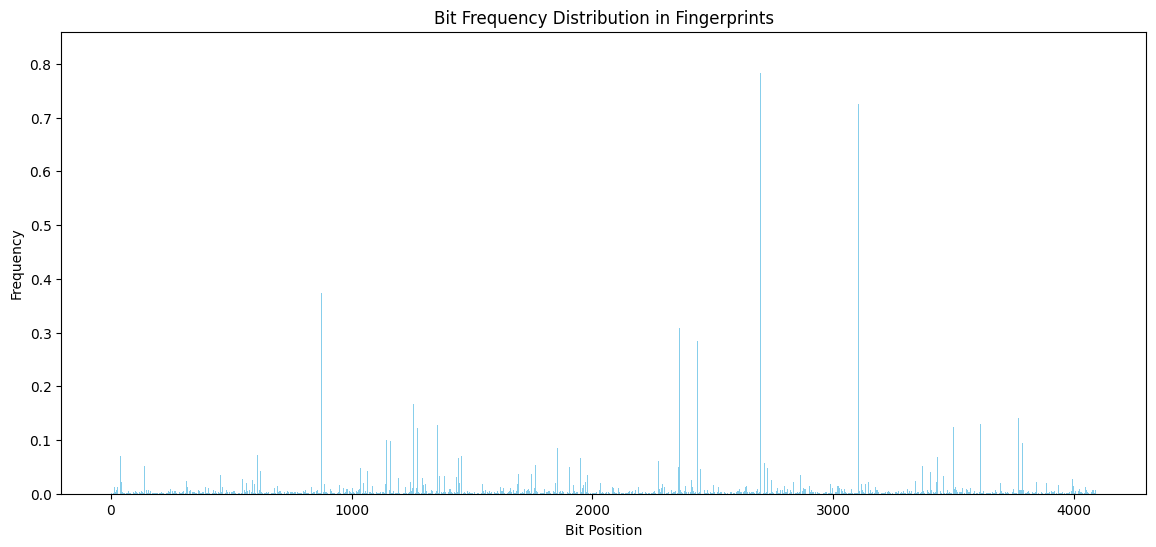
\includegraphics[width=\linewidth]{figures/background/bit-frequency-distribution-fingerprints.png}
    \caption{Bit frequency distribution of Morgan Fingerprints in GNPS dataset}
    \label{fig:bit_frequency_fingerprints}
\end{figure}

A similarity metric that takes the sparseness of these fingerprints into account is the Tanimoto similarity (i.e. Jaccard index). Using the notation by \textcite{mathieson2017computer}  the Tanimoto similarity of 2 real vectors A and B is defined as follows:
\[Tc_G(A,B) = \frac{\sum\limits^n_{i=1}{A_iB_i}}{\sum\limits^n_{i=1}{A_i^2} + \sum\limits^n_{i=1}{B_i^2} - \sum\limits^n_{i=1}{A_iB_i}}\]

For vectors containing only binary values this can be simplified as \cite{mathieson2017computer}:
\[Tc(A, B)=\frac{c}{a + b - c}\]
Where $A$ and $B$ are 2 bitvectors. $a$ and $b$ are the amount of activated bits for the 2 bitvectors respectively. The amount of bits that are activated in both $A$ and $B$ is represented with $c$. The Tanimoto similarity of two fingerprints is the ratio of shared properties to the total number of unique properties in the fingerprints \cite{mathieson2017computer}, or, in other words, the intersection over union of the 2 bit sets. Only properties that are present in one of the fingerprints are taken into account for the calculation. This makes the metric robust for sparse bitvectors.

By calculating the Tanimoto similarity of structural fingerprints (for which the properties represent the presence of unique substructures) or radial fingerprints (which has local structural properties) we can estimate the structural similarity of the underlying molecular structure.

\textcite{bajusz2015tanimoto} have benchmarked different metrics and shown that the Tanimoto similarity metric should be considered as one of the best similarity metrics on molecular fingerprints. It is still not an optimal molecular similarity metric for when the exact structures are known, as fingerprints are unable to store enough structural information. By converting the exact structure to a fingerprint, there is a loss of information \cite{kretschmer2023small}.

\subsection{MCES Distance}
\label{sec:mces_dist}

For molecular representations where we can accurately extract the molecular structure (InchI, SMILES, DeepSMILES, SELFIES), we can construct a molecular graph of the molecule \cite{wigh2022review}. Molecular graphs are labeled graphs where edges describe bonds and nodes describe atoms \cite{kretschmer2023small}. From two molecular graphs, a graphical similarity metric can then be calculated to get an accurate molecular similarity metric. 

One such graphical metric that extrapolates well to chemical structure similarity is the \ac{MCES} distance \cite{kretschmer2023small}. The MCES distance of two graphs A and B is defined as follows:
\[d_{MCES} = E_A + E_B - 2E_{MCES_{AB}}\]
Where $E_A$ is the amount of edges in graph A, and $MCES_{AB}$ is the maximum common edge subgraph of A and B, this is the largest graph for which all edges (with their corresponding end nodes) are present in A and B. Intuitively the MCES distance is the minimal amount of edges we have to remove from both graphs to get isomorphic graphs \cite{kretschmer2023small}. Or from a chemistry standpoint, by \textcite{kretschmer2023small} "the 'number of chemical reactions' required to transform one molecule into another".

Even with the optimizations proposed by \textcite{kretschmer2023small}
(e.g., They use a maximum distance upper bound.
Exact MCES distances are only calculated when they are estimated to be lower than this bound,
otherwise the upper bound is returned, termed the myopic MCES distance),
the calculation of the MCES is NP-hard and thus very compute-intensive.
When the MCES distance is used for evaluation in a machine learning molecular structure prediction setting,
this will slow down evaluation time drastically compared to a faster evaluation metric, e.g. Tanimoto similarity on fingerprints.

\section{Identifying molecules from \ac{MS/MS}}
\label{sec:relatedwork}

There have been a lot of studies on the use of Mass Spectrometry data to predict chemical structures. Table \ref{tab:relworkpapers} lists the most credited papers with their models, showing the evolution of the field of molecular structure prediction using MS/MS data.
"De novo" in this context means that a chemical structure is predicted directly without the use of candidate selection. Candidate selection models rank the chemical structures in a database by how closely they relate to the input structure. "De novo" models are able to predict a chemical representation without a reference dataset. The chemical structure can be derived by these models by only using the features learned from the training set.

\begin{table}[h]
	\setlength{\tabcolsep}{3pt}
        \renewcommand{\arraystretch}{1.5}
	\caption{
		Models predicting molecular structures from most cited papers
	}
	\resizebox{1.00\linewidth}{!}{
	\begin{tabular}{p{4cm}p{3cm}p{3cm}p{3cm}p{1cm}p{1.5cm}}
		\toprule
                \textbf{Model/Paper} & \textbf{Input Data} & \textbf{Model Output} & \textbf{Architecture} & \textbf{De Novo} & \textbf{Year Published} \\
            \midrule
		      %https://pubmed.ncbi.nlm.nih.gov/22815355/
                 FingerID \cite{heinonen2012metabolite}  & MS/MS & Fingerprints & SVMs & No & 2012 \\
                 %https://www.pnas.org/doi/10.1073/pnas.1509788112
                 CSI:FingerID \cite{duhrkop2015searching}  & MS/MS & Fingerprints & Fragmentation trees + SVMs & No & 2015 \\
                 %https://www.nature.com/articles/s41592-019-0344-8
                 Sirius 4 \cite{duhrkop2019sirius}  & MS/MS & Fingerprints & Fragmentation trees + SVMs & No & 2019 \\
                 %https://link.springer.com/article/10.1007/s11306-020-01726-7
                 MetFID \cite{fan2020metfid} & MS/MS & Fingerprints & MLP & No & 2020 \\
                 %https://www.biorxiv.org/content/10.1101/2022.12.30.522318v1
                 MIST \cite{goldman2023annotating}   & MS/MS & Fingerprints & Transformer & No & 2022 \\
                 %https://chemrxiv.org/engage/chemrxiv/article-details/6626775021291e5d1d61967f
                 DreaMS \cite{bushuiev2024emergence}  & MS/MS & Embedding Vector & Transformer & No & 2023 \\
                
                 \midrule
                 %https://pubs.acs.org/doi/10.1021/acscentsci.7b00572
                 \textcite{gomez2018automatic} & SMILES  & (latent space +) SMILES    & VAE + RNN & Yes & 2018 \\
                 %https://chemrxiv.org/engage/chemrxiv/article-details/613e83a7656369203b2a249b
                 Spec2Mol \cite{litsa2021spec2mol} & MS/MS & SMILES & CNN + GRU & Yes & 2021 \\
                 %https://www.nature.com/articles/s41592-022-01486-3
                 MSNovelist \cite{stravs2022msnovelist} & Fingerprints  & SMILES    & RNN     & Yes     & 2022 \\
                 %https://www.mdpi.com/2218-273X/11/12/1793
                 MassGenie \cite{shrivastava2021massgenie} & in silico MS/MS & SMILES & Transformer & Yes & 2021 \\
                 %https://doi.org/10.26434/chemrxiv-2023-vsmpx-v4
                 MS2Mol \cite{butler2023ms2mol} & MS/MS & SMILES & Transformer & Yes & 2023 \\
		\midrule
	\end{tabular}
	}
	\label{tab:relworkpapers}
\end{table}

% Extra sources
%https://jcheminf.biomedcentral.com/articles/10.1186/s13321-016-0116-8

\subsection{Fingerprint prediction}

One of the first models to only use tandem mass spectrometry to predict chemical features in the form of a fingerprint is \textbf{FingerID} \cite{heinonen2012metabolite}. It is a relatively simple model that first converts the peaks of the tandem mass spectrometry output to discrete binned values. These are then passed to a set of kernels in a \ac{SVM} learning model to predict structural molecular fingerprints. These fingerprints could then be used to extract certain properties of the molecule or be used as a search key to compare against a database of known molecular structures with their fingerprints (e.g. PubMed), to rank the most similar structures. 

\textbf{CSI:FingerID} \cite{duhrkop2015searching} significantly improves the methods proposed in FingerID by first computing fragmentation trees from the mass spectrometry spectra to better explain the fragmentation spectrum.
Fragmentation trees describe the fragmenting process a precursor ion underwent during mass spectrometry \cite{bocker2008towards}. The tree-like structure uses fragments as nodes and edges to stipulate that a child node is the result of the fragmented parent node. To construct such a tree,
each peak in the output spectrum after tandem mass spectrometry fragmentation is assigned the most probable chemical formula corresponding to that peak using well established algorithms such as SIRIUS (an earlier version of the further discussed SIRIUS 4) \cite{duhrkop2019sirius}.
Then the construction algorithm builds the tree to describe the peaks of fragments in the spectrum.
It takes into account the loss of small molecules during fragmentation.
These fragmentation trees are then used as input for a \ac{SVM} to predict structural molecular fingerprints in a similar way as the FingerID model.

\textbf{SIRIUS 4} \cite{duhrkop2019sirius} integrated the concepts of CSI:fingerID with the goal of making it more accessible with a \ac{GUI}. It increased the training set for the \ac{SVM} model along with built in parallelization optimizations for the database lookup algorithm using the structural fingerprints. It improved the quality of use significantly for the broader public, and is therefore often referred to as a standard for inferring molecular structures from tandem mass spectrometry spectra by database retrieval.

By binning the spectral data (as the previous papers do), a bit of information is lost as the values in each bin are squished together. \textbf{MIST} \cite{goldman2023annotating} (Metabolite Inference with Spectrum Transformers) uses another approach. It also maps a chemical formula to each peak using the SIRIUS \cite{duhrkop2019sirius} algorithm, but instead of binning the spectral intensities, it feeds these along with the chemical formula to a simple \ac{MLP} network, which outputs a feature vector for each peak. The paper discusses that these feature vectors are able to hold more information than the discretized binned values from the previous papers.
These feature vectors are then used as input for a transformer which outputs structural molecular fingerprints. A key aspect is that the relation between peaks is not explicitly fed into the model as with fragmentation trees. The multi-headed attention layers of the transformer are able to learn this relation by themselves. MIST proved capable of predicting good molecular fingerprints, but when the database retrieval part of the pipeline is taken into account CSI:FingerID seems to perform better. The MIST paper claims the CSI:FingerID model has been overfit for this custom Bayesian fingerprint retrieval method, and their model's fingerprint outputs still outperform those from CSI:FingerID.

Because these models are only able to predict molecular fingerprints
(from which the exact molecular structure can not be derived),
they are not able to predict an exact molecular structure by themselves.
A database lookup is needed to find the most similar structure. They are hence not able to predict molecular structures lying in "dark chemical space" \cite{bushuiev2024emergence}. Dark Chemical Space is a term to denote all the molecules that have not been annotated in existing databases. Annotating molecules is a very cumbersome and laborious task. Only a fraction of all the possible molecular structures are annotated. This means that these methods are only useful on a relatively small subset of molecular structures \cite{bushuiev2024emergence}.

Another way of predicting molecular fingerprints is to map the spectra from \ac{MS/MS} into an embedding vector.
From this embedding vector, a simple feed-forward model can then be trained to extract the fingerprint.
This is exactly what is achieved with \textbf{DreaMS} \cite{bushuiev2024emergence} (Deep Representations Empowering the Annotation of Mass Spectra).
It uses a BERT-style encoder \cite{devlin2018bert} to encode spectra to an embedding space.
This is done in a self-supervised manner, where during training a portion of the spectrum is masked and the model is tasked to predict the masked peaks.
The model maps the spectra into an embedding space.
This embedding space can then be fine-tuned for multiple tasks, such as structural fingerprint prediction.
This is very promising as the biggest bottleneck for training these models is the lack of annotated data.
Because the DreaMS encoder can be trained on spectra only, it can also use all the unannotated spectra available, thereby increasing the representational capacity of the model. The fine-tuned structural fingerprint prediction using DreaMS embeddings showed to be outperforming the predictions from MIST.

\subsection{Textual representation prediction}

Models that are able to directly predict a molecular representation, from which the molecular structure can be easily derived (e.g. SMILES) are called "de novo" models. They are able to predict "new" molecules that aren't present in any databases. Most of these representations are textual, meaning the recent advances in the field of natural language processing can be used to predict them.

One of the first papers that explored the auto-regressive generation of textual representations is by \textcite{gomez2018automatic}.
Their proposed model consisted of a \ac{VAE} that was able to encode a SMILES string to a latent space.
A \ac{RNN} could then decode the latent space back into a SMILES string.
They also had a predictor that could derive properties from the encoded latent space (similar to a fingerprint predictor from the embedding in DreaMS).
Because the model was able to predict valid smiles from any point in the latent space, modified or completely random latent vector could then be fed through the decoder to get a de novo SMILES string. It showed the power of autoregressive models for de novo molecular structure generation.

This concept was used in \textbf{Spec2Mol} \cite{litsa2021spec2mol}. They firstly train an auto encoder using \acp{GRU} that is able to encode and decode smiles to and from an embedding. Once the model is trained, they train a new encoder using a \ac{CNN} that maps spectral data to the corresponding embedding using the pre-trained encoder to generate the embeddings as labels. Then, the encoder that encodes spectral data to the embedding is combined with the pre-trained decoder that decodes this embedding to a SMILES string.
This pipeline can map a spectrum from \ac{MS/MS} to a textual molecular representation. The key aspect they tackle is the lack of spectral data, because the first auto encoder can be trained unsupervised, a lot more data is available.

Instead of using a pre-trained embedding, \textbf{MSNovelist} \cite{stravs2022msnovelist} used the fingerprints of the CSI:FingerID model, widely considered to be the most powerful structural fingerprint prediction model at the time. It used a \ac{RNN} as a decoder, but instead of decoding a latent space vector, it used structural fingerprints from CSI:FingerID. A SMILES representation of a specific fingerprint can then be predicted from a \ac{MS/MS} spectrum. Because the model is trained on structural fingerprints, and any SMILES string can be easily converted to a structural fingerprint, only SMILES are needed to train the model. A big drawback is the fact that structural fingerprints do not contain enough information by themselves to describe a molecular structure (e.g. inability to distinguish certain isomers), the model will thus never be able to perform perfectly \cite{kretschmer2023small}.
The results from the paper do show that, for small molecules, the model is able to predict a reasonable structure for more than half of the spectra in its test set.

\textbf{MassGenie} \cite{shrivastava2021massgenie} tries to solve the lack of data problem in another way. The opposite problem (predicting fragmented \ac{MS/MS} spectra from a molecular representation) is much more feasible because the strengths of bonds are mostly known. Bonds with weaker strength are more likely to be the fragmentation point. They use this to first generate a lot of in silico spectra from structural libraries. In silico spectra are \ac{MS/MS} spectra that are generated from a molecular representation (SMILES in this case). The result is a very large set of spectra that can be used to train the original problem. They then handle the spectrum to molecular representation mapping as a language translation problem, Transformers are known to be very powerful for this task. MassGenie uses a autoregressive transformer network to predict SMILES strings. 
To further improve the prediction and have a higher chance of finding the correct molecular representation, they feed the output SMILES string of the transformer to a previously published model that generates candidate SMILES strings, SMILES that are very similar but not identical. This model is called VAE-Sim \cite{samanta2020vae} and was trained unsupervised using the \ac{VAE} network architecture. These candidate SMILES strings (along with the original prediction) are then matched separately to the true SMILES string.
Because the spectral data used to train the model is in silico data, it is not as generalizable to real world (in vivo) data. However, the model does seem to show competitive results compared to previously discussed models.

Instead of generating in silico spectra, \textbf{MS2Mol} \cite{butler2023ms2mol} used an improved model architecture to more efficiently use the training data. It uses a BART-style \cite{lewis2019bart} transformer. BART-style transformers use a similar BERT-style encoder with an auto-regressive decoder.
A transformer decoder is used, which can be iteratively called to auto-regressively generate SMILES characters. The model is trained end-to-end. It leverages its power by taking the following concepts into account: 
(1) A byte-pair encoding tokenizer is pre-computed on the SMILES of a large unlabeled dataset to group common substructures of SMILES as one token. This will improve the models output and reduce the amount of invalid SMILES.
(2) The precursor mass of the unfragmented compound is given along with the spectrum as input for the model. To reduce overfitting, this precursor mass is masked half the time during training.
(3) Instead of using binned values from the spectrum, the intensities of the peaks are split into their real part and their fractional part. The fractional part is then rounded to a certain precision. Each peak is represented as a token pair of these two values. This way the peaks of the spectrum are represented using a minimal set of token pairs, while still holding more information than binned spectra methods. 
(4) By using Beam Search on the decoder, the model is able to rank predictions. Allowing the model to only output the top-ranked predictions.
From the results in the paper, MS2Mol seems to outperform all other models previously discussed on de novo test sets. On test sets such as CASMI \cite{schymanski2017critical} for which retrieval methods are optimized, it seems that the model is still outperformed by CSI:FingerID.

\section{Standardization with MassSpecGym}
\label{sec:massspecgym}

The biggest bottleneck discussed in all papers above is the lack of (annotated) (open-source) spectral data. While many models try to optimally use the data available, they still suffer with the small datasets. Molecular structure prediction is proven to be a difficult task \cite{kretschmer2023small}, the lack of high-quality and high-quantity datasets do not make this easier.
On top of that, the mentioned papers do not use a standardized way to benchmark results. By using different evaluation metrics, different datasets, and so on, it is very hard to compare the performance of the models. It seems that the papers mostly cherry-pick the settings for which their model outperforms the others. This shows that there is a clear need for a standardization within the field.
While many use already standardized datasets and evaluation metrics from the molecular structure retrieval domain (e.g. CASMI \cite{schymanski2017critical}), these metrics are not optimal for evaluating de novo structure prediction models. They do not take molecular structures from the "dark chemical space" into account, for which de novo models should be used. It is then only logical that de novo models can't seem to outperform the molecular retrieval models that are optimized for their datasets.

To further improve the domain of de novo molecular structure prediction, specific standardized datasets of unknown compounds along with standardized evaluation metrics are required.
This is exactly what \textbf{MassSpecGym} \cite{bushuiev2024massspecgym} tries to achieve. It proposes the largest open-source dataset with the same name, along with an ImageNet-like \cite{5206848} competition leaderboard with standardized evaluation metrics to make the domain more accessible to a wider public.
With this dataset, they propose three main challenges:
\begin{description}
    \item[De novo molecule generation] Predicting molecular structures from tandem mass spectrometry data. (e.g. MS2Mol)
    \item[Molecule retrieval] Retrieving most-probable molecular structures using database lookup methods. (e.g. CSI:FingerID)
    \item[Spectrum Simulation] Predicting spectral data from molecular structures, the exact inverse problem of de novo molecule generation. (e.g. MassGenie in silico spectrum generation)
\end{description}

\subsection{MassSpecGym Dataset}
\label{subsec:massspecgymdataset}
The MassSpecGym dataset consists of the largest available spectral libraries: MoNA \cite{mona}, MassBank \cite{horai2010massbank}, GNPS \cite{wang2016sharing} and their in-house data \cite{brungs2024efficient}.
These datasets are combined and deduplicated.
Then, all the low quality spectra are filtered out using a standard procotol by \textcite{de2023reproducible} along with some additional filters such as only keeping spectra with an m/z < 1000. After filtering, estimated instrument noise is removed from the spectra. The result is a large dataset (231,000 entries) that contains only high-quality spectral data along with their different molecular representations. This combination of different datasets should combat the problem of only having data from a certain domain described by \textcite{kretschmer2023small}. They also provide even bigger unlabeled datasets for both spectra (24,000,000 entries) and molecules (3 datasets: 1,000,000 entries, 4,000,000 entries and 118,000,000 entries).

Another problem that many of the discussed models experience is leakage \cite{bushuiev2024massspecgym}. Certain molecules used during training are too similar to molecules in the test set. This inflates the results but gives a very distorted image of the model's performance as it will perform much worse on unseen dissimilar molecules. To solve this problem, the train, validate and test folds are clustered by calculating the \ac{MCES} distance between the molecules. This ensures that all molecules have a minimal \ac{MCES} distance (10 in the case of MassSpecGym) to the molecules in other folds. The spectra are also "stratified by instrument types, collision energies, ionization adducts, and the frequency of the molecules in the entire dataset" \cite{bushuiev2024massspecgym} to reduce variance.

\subsection{De Novo Models}
\label{subsec:massspecgymmodels}

The MassSpecGym paper \cite{bushuiev2024massspecgym} presents 3 baseline models for de novo molecular structure prediction from \ac{MS/MS} data:
\begin{description}
    \item[Random chemical generator] An algorithm that uses combinatorial and graph theory algorithms which is out of the scope of this thesis.
    \item[SMILES transformer] Similar to the method used in MS2Mol \cite{butler2023ms2mol}, this model uses a transformer with an autoregressive decoder to predict SMILES. A tokenizer is also precomputed by using a byte-pair encoding on the SMILES of the large unlabeled molecule dataset.
    \item[SELFIES transformer] This model also uses a transformer with an autoregressive decoder but instead of predicting SMILES, it predicts SELFIES. Because SELFIES are always syntactically and chemically viable, no byte-pair encoding is used.
\end{description}
Both the SMILES transformer and SELFIES transformer use a greedy sampler (explained in the next Section \ref{sec:samplingmethods}) that outputs the token with the highest probability iteratively when only one prediction is required. When more predictions are required, they sample from the (with temperature scaled) probabilities from the decoder's output.

The models are evaluated by measuring accuracy (if the prediction exactly matches the label), \ac{MCES} distance (on the molecular graphs) and Tanimoto similarity (on the fingerprints that can be derived from the structure). Because the problem at hand is very hard, allowing the model to only predict one molecular representation (top-1) is very strict. A relaxed version, for which the model is able to predict 10 molecular representations (top-10), is also used. The metrics are calculated for all predictions, but only the best score for each metric is kept.

The baseline models in the MassSpecGym paper perform very poorly, they all have a top-10 test accuracy of 0\%. The algorithmic model even has the best performing predictions in terms of top-1 MCES distance. Overall, it is indicated that there is still a lot of room for improvement. 

\section{Autoregressive sampling methods}
\label{sec:samplingmethods}

The best performing de novo molecular structure predicting models use textual molecular representations (e.g. SMILES) as output \cite{litsa2021spec2mol, shrivastava2021massgenie, butler2023ms2mol}.
They are generating autoregressively by a sampling function, meaning they are generated token by token sequentially. The decoder takes the encoded \ac{MS/MS} data and already generated tokens (called context) as input, and outputs a probability for each token in the vocabulary. This probability describes how likely the token $x_i$ is to be following the context tokens $y_{1}, y_{2}, \dots, y_{i-1}$. 
\[P(y_i | y_{i-1},y_{i-2},\dots,y_{1})\]
This probability distribution is calculated by the Softmax function $\sigma$ \cite{nwankpa2018activation} over the decoder's output vector $z$ (logits).
\[y_i = \sigma(z_i) = \frac{exp(z_i)}{\sum\limits_{j=1}^{||z||} exp(z_j)}\]
To scale the probability distribution (and thus influence the behavior of a sampler), a temperature parameter $T$ can be introduced. 
\[y_i = \sigma(z_i, T) = \frac{exp(\frac{z_i}{T})}{\sum\limits_{j=1}^{||z||} exp(\frac{z_j}{T})}\]
A low temperature $T$ value will increase the probability for the most likely following token and decrease the probabilities of the less likely tokens. A high temperature will give a more uniform distribution where the less probable following tokens are given a higher probability. The higher the temperature, the more random the tokens that the sampler will predict. 

A naive sampling method would just sample with the output probabilities from the model (optionally scaled with a temperature $T$). \textcite{holtzman2019curious} has shown, however, that doing this with text generating models results in repetitive and degenerate text. They proclaim that using a specialized sampling method increases the quality of the predictions significantly.
The most used sampling methods are listed below \cite{holtzman2019curious}:
\begin{description}
    \item[Greedy sampling] This sampling method always returns the token with the highest probability. In text generation this will often lead to repetition.
    \item[Top-k sampling] Here, only the top-k tokens with the highest probabilities are taken into account. The method samples from their probabilities that are rescaled between them. It is a method to remove the low probability of the less likely tokens to be sampled.
    \item[Top-p / Nucleus sampling] In this sampling method, the top x tokens are calculated for which their cumulative probability exceeds a parameter p, with x kept as low as possible. Again, the method samples from the rescaled probabilities of the top x tokens. It is a more balanced method for removing the probability for less likely tokens to be sampled.
    
    \item[Beam Search] \cite{freitag2017beam} This is a greedy breadth-first search algorithm that maximizes a scoring function.
    For this method, a beam width parameter $b$ dictates the search space. At each time step, $b$ partial predictions are stored.
    Only the probabilities for the next tokens of these $b$ partial predictions are calculated.
    Each next token is then given a score using a scoring function that takes the context into account based on the cumulative probability.
    The tokens for which the scores are the highest are stored along with their context as new partial predictions.

    An example of a scoring function that scores a partial prediction consisting of a vector of tokens $y$ with length $L$ is:
    \[score(y) = \frac{1}{L^a} \sum\limits_{t=1}^{L}log\ P(y_t | y_{t-1},\dots,y_{1})\]
    Because the scoring function is based on the cumulative probability, a length normalization (adjustable with parameter $\alpha$) is included to prevent the sampler from preferring short sequences.
    
\end{description}

Naive, top-k and top-p sampling introduce some randomness that allows them to generate a new prediction when called multiple times, while greedy sampling (1 prediction) and beam search (predictions = beam width) are deterministic and will return the same prediction(s).

\textcite{stravs2022msnovelist} did a comparative study for the different sampling methods with their MSNovelist model and found Beam Search to be the best performing method for predicting SMILES.

\chapter{Aims}
\label{chap:aims}

De novo molecular structure prediction from \ac{MS/MS} research is still at a very early stage.
A few attempts were made to adopt the already more established research from the \ac{NLP} field regarding the use of deep generative models for text prediction, to predict SMILES.
Many decisions made to the model architecture were made by copying earlier research on large language models.
Because we are working in a different research domain, and the textual molecular representations have entirely different properties compared to natural language,
many of these decisions could be questioned.
Only now that a standardized dataset and benchmark (MassSpecGym) was released, it is possible to optimize these models.
Because MassSpecGym is the biggest available dataset with high quality spectra and it implements data leakage prevention methods, it is the preferred dataset for this thesis.
The aim of this thesis is not to train the best de novo molecular structure predicting model,
only to benchmark the currently most used methods in the de novo string-based molecular structures prediction domain.
This way, further research can adopt these findings and steer away from the standards of the natural language processing field.

The following experiments are performed in this thesis:

\begin{description}
    \item[Replicate MassSpecGym results]
    To establish a common baseline for the experiments and because the trained models are not available, the de novo models from the MassSpecGym paper \cite{bushuiev2024massspecgym} have to be retrained.
    A lot of the optimal hyperparameters from the paper's results are on the edge of its search space.
    To verify that these are the optimal hyperparameters, a grid search with an extended search space has to be replicated.
    In this thesis only a grid earch for the SMILES de novo model is performed.
    
    \item[Benchmark autoregressive samplers]
    There are a lot of different auto-regressive sampling algorithms from the \ac{NLP} domain.
    The limited research that exists to compare these algorithms for string-based molecular structures was done on outdated models and domain specific datasets \cite{stravs2022msnovelist}.
    For this experiment the different samplers from section \ref{sec:samplingmethods} are benchmarked on the SMILES model.
    
    \item[\acf{BPE} as pretraining]
    One of the biggest challenges for SMILES predicting models is the validity of the output. Syntax or chemical errors lead to invalid SMILES.
    To combat this, the de novo SMILES model from MassSpecGym uses a tokenizer that pre-computes its vocabulary with \ac{BPE} on a large unlabeled dataset of SMILES.
    The model can then use the learned patterns from the tokenizer to train and predict SMILES.
    This can be considered a way of pre-training the model.
    A few key question to be considered with this method are: 
    (1) How does using \ac{BPE} impact performance?
    (2) Can we improve the pre-training by using a larger unlabeled dataset?
    (3) Does this method influence over-fitting?
    This experiment will try to answer these questions by benchmarking performance of SMILES models trained with different tokenizers.

    \item[Augmentation]
    A recurring problem for training de novo molecular structure predicting models, is the lack of training data.
    To combat this without actually measuring new data, data augmentation can be used. 
    Two augmentation methods are benchmarked in this thesis.
    (1) Because multiple SMILES can represent the same molecule, we can use these SMILES synonyms as label augmentation.
    (2) A different precursor mass can cause the mass spectra of identical molecules to be shifted.
    We can use this to our advantage to mimic new spectra by applying a small identical shift to the peaks.
    This way the training spectra can be augmented.
    This experiment measures the performance and overfitting by using these augmentation methods.

    \item[Molecular representations]
    Different string-based molecular representations have been published (see section \ref{sec:molrepr}) to describe a molecular structure.
    By comparing performance on identical models trained with different string-based molecular representations,
    the goal of this experiment is to find the best string-based molecular representation for de novo molecular structure prediction.
     
\end{description}


\chapter{Results}
\label{chap:results}

The following sections briefly describe the experimental setup, before showing the results for each experiment discussed in Chapter \ref{chap:aims}.
These experimental results are also discussed in this chapter.


\section{Hyperparameter gridsearch}

As a first experiment, the de novo SMILES MassSpecGym model was reproduced and extended with a larger gridsearch.
The extended hyperparameter search grid for the retrained SMILES models, along with MassSpecGym's grid search results, is presented in Table \ref{tab:gridsearch}.
The hyperparameter combination that achieved the lowest validation loss is highlighted in bold.

\begin{table}[h]
	\caption{
		Gridsearch MassSpecGym vs Gridsearch Thesis for the de novo SMILES transformer (lowest validation loss models in bold).
	}
    \resizebox{\textwidth}{!}{
	\begin{tabular}{p{6cm}W{c}{4cm}W{c}{4cm}}
		\toprule
                \textbf{Hyperparams} & \textbf{MassSpecGym} & \textbf{Thesis Gridsearch} \\
            \midrule
                Learning Rate & $\mathbf{3\cdot 10^{-4}}, 1\cdot 10^{-4}, 5\cdot 10^{-5}$ & $1\cdot 10^{-3}, 3\cdot 10^{-4}, \mathbf{1\cdot 10^{-4}}$\\
                Batch Size & $512, \mathbf{1024}$ & $\mathbf{512}, 1024, 2048$ \\
                $n$ predictions & $\mathbf{10}$ & $\mathbf{10}$ \\
                Transformer hidden dimensionality & $\mathbf{256}, 512$ & $\mathbf{128}, 256, 512$ \\
                Number of attention heads & $\mathbf{4}, 8$ & $2, 4, \mathbf{8}$ \\
                Number of encoding layers & $\mathbf{3}, 6$ & $\mathbf{2}, 3, 4$ \\
                Number of decoding layers & $\mathbf{4}$ & $2, 3, \mathbf{4}$ \\
		\midrule
	\end{tabular}}
	\label{tab:gridsearch}
\end{table}

By retraining with the extended search grid, several models were found that outperformed the retrained model with the best hyperparameter combination from MassSpecGym, according to the validation loss.
Note that the number of predictions (i.e. top-1 or top-10) is kept constant as this does not influence the loss.
There is a substantial difference between the optimal hyperparameters from the retrained gridsearch and MassSpecGym's results.
Because the loss function does not accurately describe the model's ability to predict de novo molecules from \ac{MS/MS},
a naive sampler, that just iteratively samples from the model's output distribution (as described in Section \ref{sec:stochastic_samplers}), was used to predict SMILES on the validation set.
The evaluation of the SMILES predictions from both models using this sampler can be found in Figure \ref{fig:gridsearch_vs_paper}.
The \ac{MCES} distance on the SMILES and Tanimoto similarity on the converted fingerprints are calculated in the strict (top-1) and more relaxed (top-10) evaluation settings.
The top-1 and top-10 exact match accuracy for both models is (close to) zero and was therefore excluded from Figure \ref{fig:gridsearch_vs_paper}.

\begin{figure}[h]
    \centering
    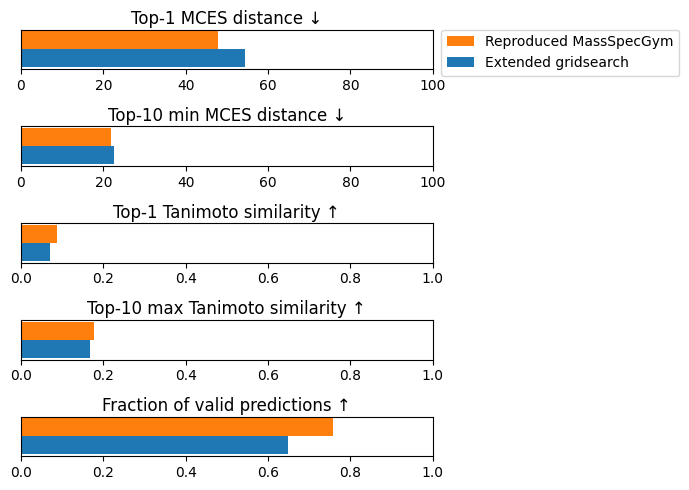
\includegraphics[width=0.8\textwidth]{figures/results/gridsearch_vs_paper.png}
    \caption{Performance comparison between the retrained SMILES model from the MassSpecGym paper versus the lowest validation loss SMILES model from the gridsearch, evaluated on the validation set.}
    \label{fig:gridsearch_vs_paper}
\end{figure}

It is clear that the retrained SMILES model from MassSpecGym outperforms the model with the lowest validation loss on every metric.
This shows that there is a discrepancy between the loss function and the evaluation metrics as lower validation loss does not necessarily indicate better predictions.
A big contributing factor to this performance difference is the fact that the retrained MassSpecGym model is able to predict 10\% more valid SMILES, as invalid SMILES have the maximum MCES distance and zero Tanimoto similarity.
The validity of the SMILES prediction could rely on the sampler and the temperature scaling of the output distribution. This is tested in the next experiment.


\section{Samplers benchmark}

To test how much temperature scaling and different samplers can influence model performance, different samplers were used to predict the validation set of the model with the lowest loss from Table \ref{tab:gridsearch}.
For this experiment, the Tanimoto similarity was directly correlated to the MCES distance and will thus not be shown in the plots.
All performance differences shown with the MCES distance always show the same relative Tanimoto similarities.

Firstly, the influence of temperature scaling is tested using the naive sampler for the top-1 and top-10 settings.
These results are shown in in Figure \ref{fig:naive_and_greedy}.
Because this temperature difference will influence the randomness of the sampler's predictions, a simple greedy sampler that always predicts the most likely token is shown as a deterministic baseline.
This greedy sampler will always predict the same SMILES and can thus only be evaluated in the top-1 setting.

\begin{figure}[h]
    \centering
    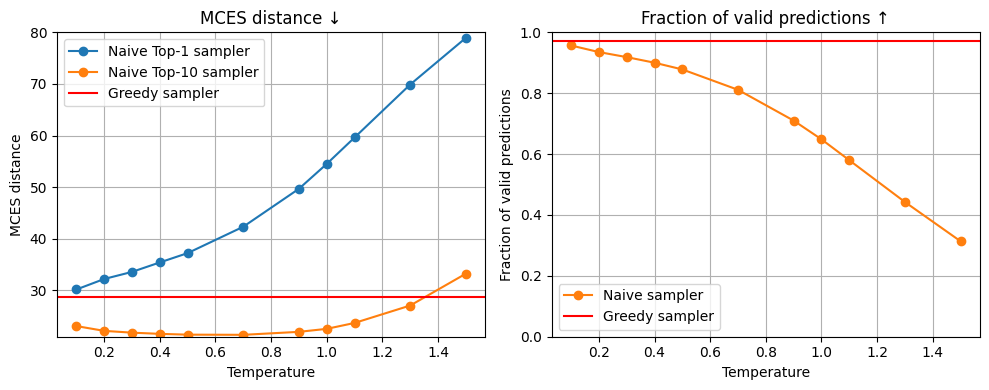
\includegraphics[width=0.95\textwidth]{figures/results/samplers/naive_and_greedy.png}
    \caption{Evaluation of the naive sampler with different temperatures on the validation set.}
    \label{fig:naive_and_greedy}
\end{figure}

From Figure \ref{fig:naive_and_greedy}, it is clear that the naive sampler performs poorly when only one prediction is evaluated (top-1).
Increasing the randomness (by increasing the temperature) for the top-1 naive sampler, only worsens the MCES distance.
As expected, the top-1 naive sampler's MCES distance converges to that of the greedy sampler as the temperature approaches zero, since extremely low temperatures force the model to only predict the most likely token.

The naive sampler benefits greatly from its randomness with top-10 evaluation, by performing better than the greedy sampler according to the MCES distance.
It shows to have an optimal temperature around $0.7$, for this SMILES model.
A higher temperature increases the randomness of the sampler too much, causing the amount of valid predictions to drop.
A lower temperature starts to force the predictions towards the greedy sampler.
These results shows that, with the temperature parameter, there is a tradeoff to be made between exploitation (low temperature) and exploration (high temperature).
The optimal temperature will depend on which evaluation setting is used.
In top-1 evaluation, each invalid prediction is penalized; therefore, exploitation, which maximizes the number of valid predictions, is important.
With top-10 evaluation, if at least one of the ten predictions per spectrum is valid, the other invalid predictions are not penalized. This gives the sampler room for exploration.
This explains the results in Figure \ref{fig:naive_and_greedy}, the greedy sampler maximizes exploitation and thus outperforms the naive sampler in the top-1 evaluation setting.
In contrast to the naive sampler, the greedy sampler is incapable of exploring multiple predictions.
Figure \ref{fig:naive_and_greedy} shows that exploration does result in better predictions, but less valid predictions, allowing the naive sampler to perform better with top-10 evaluation.

\subsection{Stochastic Samplers}

The randomness of the naive sampler can be tweaked using samplers such as top-k and top-p (nucleus sampling) as described in Section \ref{sec:samplingmethods}.
Because the stochastic samplers only benefit from their randomness when evaluating in a top-10 setting, only these results will be shown on the plots.
The temperature has shown to influence performance, therefore, a temperature search was conducted for each sampler with different parameters $k$ or $p$, where the optimal temperature (according to the lowest MCES distance) was selected.
This ensures that only the best results are shown for each the sampler with its parameter.
For completeness, the top-1, along with the temperature search results can be found in the Appendix Section \ref{sec:sampler_full_results}.

\begin{figure}[h]
    \centering
    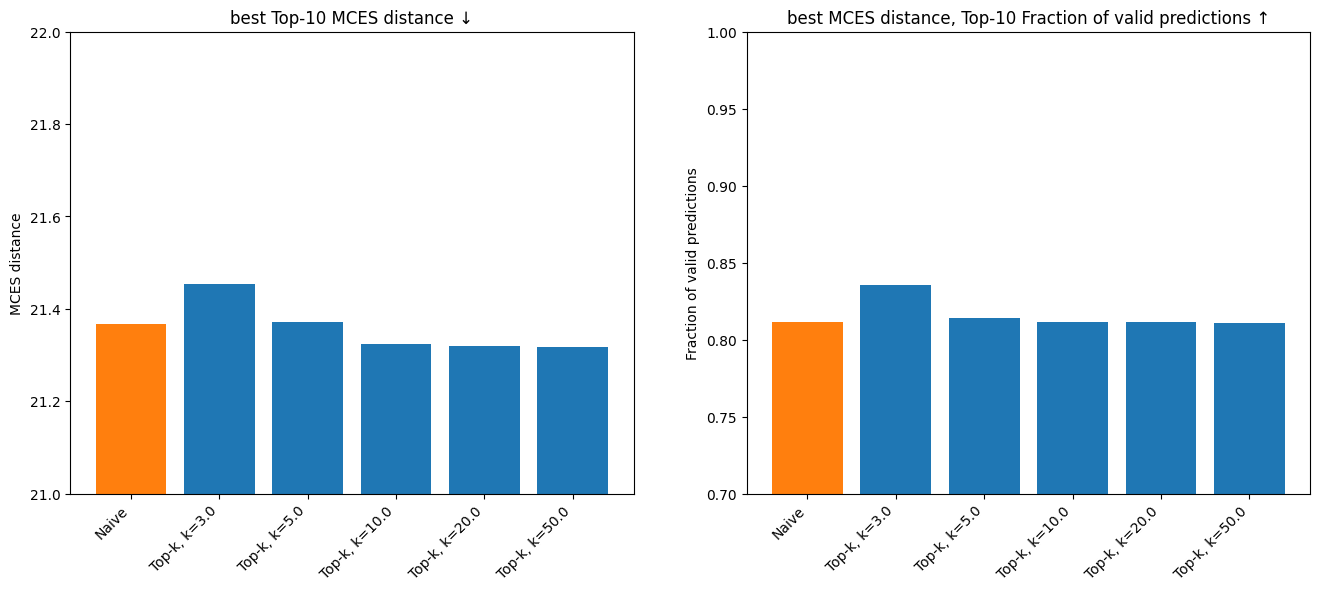
\includegraphics[width=0.85\textwidth]{figures/results/samplers/top-k.png}
    \caption{Evaluation of the (top-10, temperature optimized) top-k sampler and naive sampler on the validation set.}
    \label{fig:top-k}
\end{figure}

Figure \ref{fig:top-k} shows the performance of the top-k sampler with ranging values for $k$, top-10 evaluated on the validation set.
This figure shows that top-k sampling can slightly improve performance compared to the naive sampler when $k > 5$.
When the sampler gets limited too much, with a low $k$, it performs slightly worse. 
Note that the y-axis is scaled for visibility, the improvement is very small.

\begin{figure}[h]
    \centering
    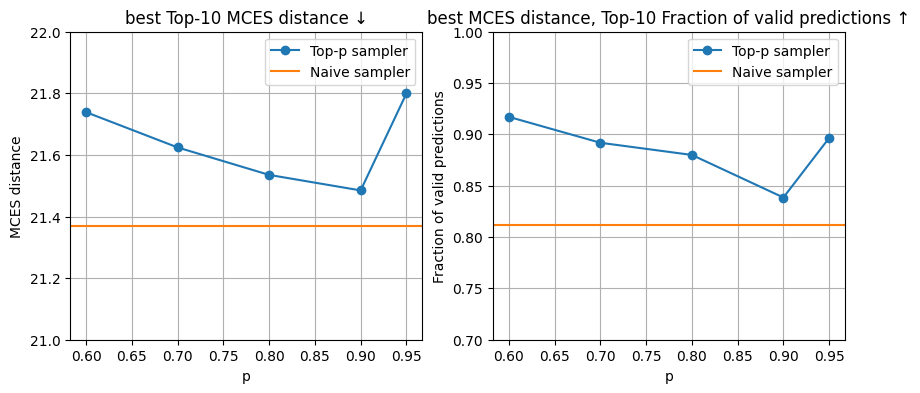
\includegraphics[width=0.85\textwidth]{figures/results/samplers/top-p.png}
    \caption{Evaluation of the (top-10, temperature optimized) top-p sampler and naive sampler on the validation set.}
    \label{fig:top-p}
\end{figure}

Figure \ref{fig:top-p} shows the performance of the top-p (nucleus) sampler for different values of $p$, top-10 evaluated on the validation set.
With top-k, limiting the randomization seems to slightly improve performance of the sampler, Figure \ref{fig:top-p} shows that this does not hold for the top-p sampler.
Overall, these randomization limiting samplers do not considerably improve the naive sampler's performance.

\subsection{Deterministic Samplers}

The beam search sampler is a deterministic sampler that improves upon the greedy sampler by increasing its search space to find multiple predictions as explained in Section \ref{sec:samplingmethods}.
Figure \ref{fig:beam-search} shows its performance for different search space sizes (beam widths).
The length regularization parameter $\alpha$ from the scoring function was also benchmarked for different beam widths but showed to have no influence on performance.
Only when large values were used ($\alpha > 10$), performance tanked to very poor results.
Forcing the sampler to predict longer token sequences with parameter $\alpha$ thus only hinders performance.

\begin{figure}[h]
    \centering
    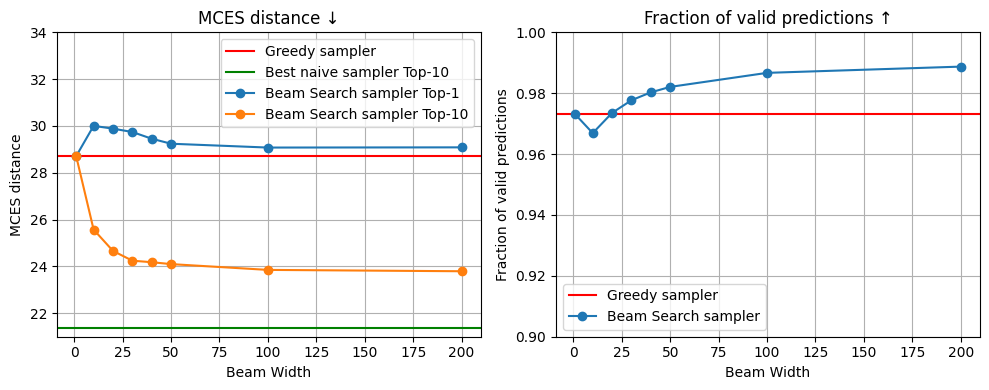
\includegraphics[width=1.0\textwidth]{figures/results/samplers/beam_search.png}
    \caption{Evaluation of the beam search sampler compared to the greedy and naive sampler on the validation set.}
    \label{fig:beam-search}
\end{figure}

Figure \ref{fig:beam-search} shows that the top-1 and top-10 MCES distance for the beam search sampler improves with increased search space as expected.
The spike in MCES distance and fraction of valid predictions on the first data point is because the beam width is 1, meaning it is essentially the same as the greedy sampler.
There is a clear performance difference between the top-1 and top-10 evaluation settings, indicating that the prediction with the highest score is often not the prediction with the lowest MCES distance.
This shows that the scoring function, and thus the output probabilities from the model, are not optimal for extracting the correct molecular structure.
This again indicates a flaw with the loss function, for which the model was optimized.

These suboptimal output probabilities also explain why the beam search sampler, which is inherently better than the greedy sampler at exploiting the model's output, performs worse in the top-1 setting than the greedy sampler.
This exploitation is clearly visible on the fraction of valid predictions plot in Figure \ref{fig:beam-search}, where the best scoring prediction from the sampler (with a beam width > 1) is always a valid molecule.

The top-10 MCES distance from the beam search sampler is still notably worse than the best top-10 naive sampler results, showing that for top-10 evaluation exploration is still preferred over exploitation.

Overall, from these results, the greedy sampler seems to perform best for the top-1 evaluation setting, while the naive sampler excels in the top-10 evaluation setting.
For all the following experiments in this thesis, the greedy and naive samplers are only used for the top-1 and top-10 evaluation setting respectively.

\section{\ac{BPE} as pretraining}

The previous experiment used a SMILES de novo model with a vocabulary, precomputed using \ac{BPE} on the unlabeled dataset with 4,000,000 SMILES from MassSpecGym.
To measure the influence of the \acf{BPE} on the model's performance, in this experiment, SMILES models were trained with different tokenizers.
These tokenizers only differ in vocabulary and, consequently, vocabulary size.
The training hyperparameters are kept the same for all models for consistency.

A simple tokenizer that does not pre-compute any substrings with \ac{BPE} in its vocabulary was used to train a baseline model.
The other tokenizers used MassSpecGym's unlabeled SMILES datasets of different sizes.
These datasets are further referred to as 4M and 118M, for the datasets with 4,000,000 and 118,000,000 SMILES respectively.
Using these unlabeled datasets can be seen as a form of pretraining, where frequently occurring substrings are captured as single tokens in the vocabulary.
All tokenizers, pre-computed with \ac{BPE}, also use the training SMILES in its \ac{BPE} corpus.
One tokenizer only used the SMILES from the training set to compute the \ac{BPE} patterns.
This model is a \ac{BPE} baseline to see how using the unlabeled datasets can influence performance.

For the 4M and 118M dataset, a second tokenizer was pre-computed where the \ac{BPE} algorithm was given a more strict cut-off for grouping characters, by increasing the minimal frequency parameter from 2 (the default value) to 10.
Lastly, because the vocabulary size of the 118M tokenizer reached the algorithm's threshold, a tokenizer was computed on the 118M dataset where computation halted as soon as the vocabulary reached the size of 5200 (equal to the vocabulary size of the 4M tokenizer). 

Figure \ref{fig:bpe} shows the evaluation of the models trained with different \ac{BPE} tokenizers, using the greedy sampler and the best naive sampler for the top-1 and top-10 evaluation settings respectively.
A new evaluation metric, the fraction of novel predictions, can be seen in the last plot.
It shows the fraction of valid predictions that are not identical to a molecule in the training set.
This measures how much the model is able to predict unseen SMILES as a metric to quantify overfitting.
The complete temperature search for the naive top-10 sampler can be found in the Appendix Figure \ref{fig:bpe_appendix}.

The most notable result from Figure \ref{fig:bpe} is that models trained with a \ac{BPE} tokenizer have more valid predictions.
Using \ac{BPE} does indeed succeed in reducing invalid predictions, achieving its intended purpose.
A huge drawback however, can be seen when looking at the fraction of novel predictions.
Using \ac{BPE} with default parameters nearly halves the number of novel predictions compared to the model trained with a non-BPE tokenizer, which indicates that using \ac{BPE} increases overfitting.

The \ac{BPE} 4M tokenizer is used in MassSpecGym's de novo SMILES model.
Figure \ref{fig:bpe} shows that it has the best performance looking at the MCES distance and Tanimoto similarity, it also achieves one of the highest number of valid predictions compared to the other tokenizers.
The poor amount of novel predictions does question if this result is due to overfitting, as more than half of its predictions are identical to molecules from the training set.

\begin{figure}[h]
    \centering
    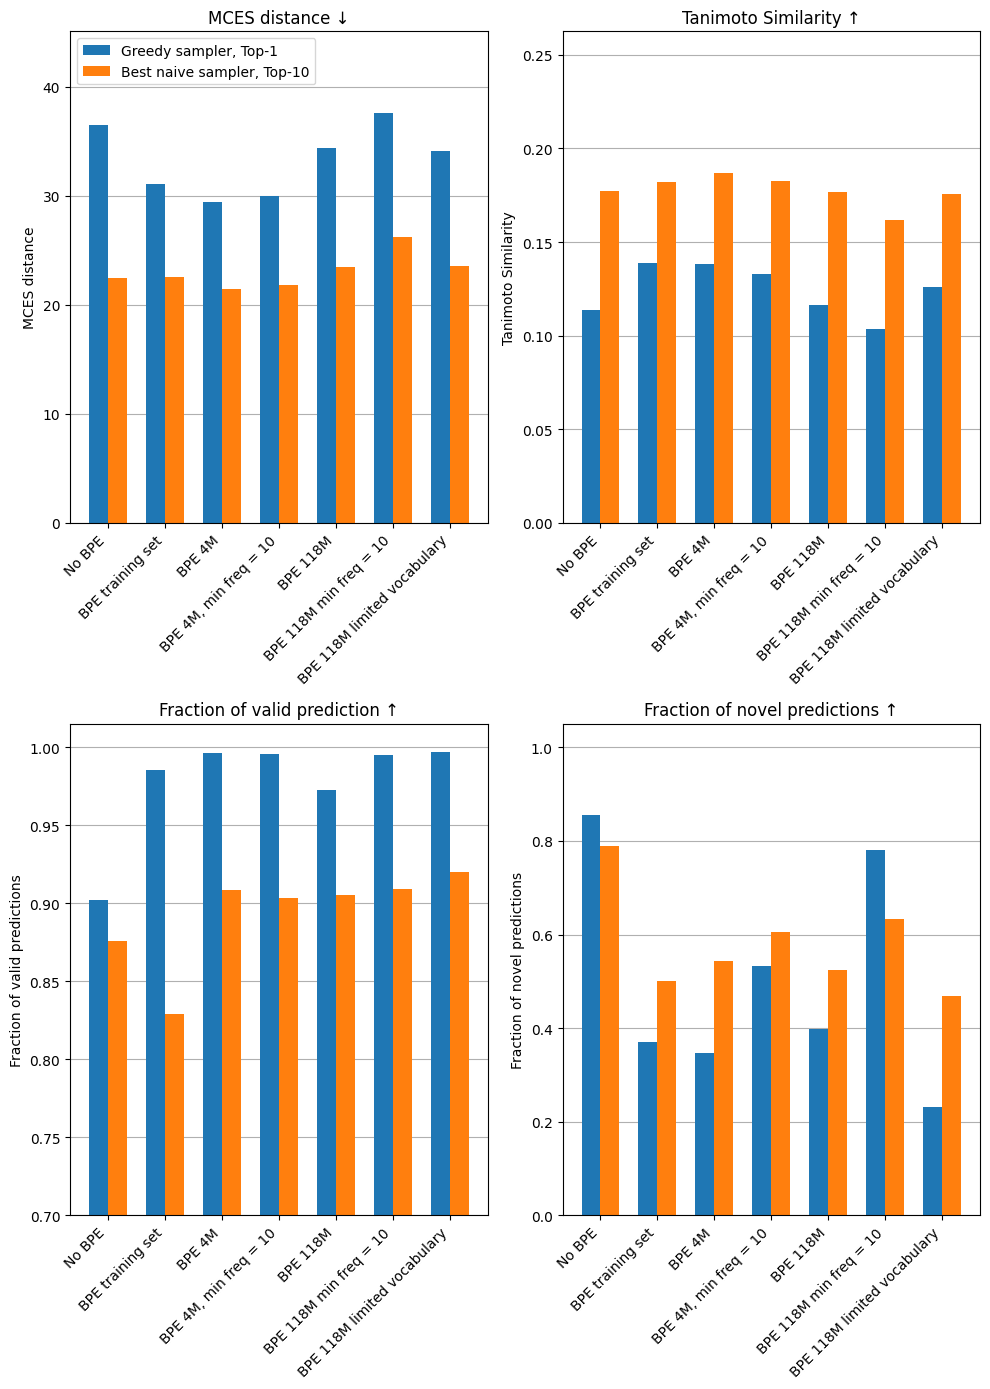
\includegraphics[width=0.79\textwidth]{figures/results/bpe_with_tanimoto.png}
    \caption{Evaluation on the validation set of SMILES models trained with different Byte-Pair encoded tokenizers.
    Note that the y-axis of the fraction of valid predictions plot does not start at zero for readability.}
    \label{fig:bpe}
\end{figure}

A strange result is that the use of the larger 118M dataset does not improve performance compared to the 4M dataset when comparing MCES distance and Tanimoto similarity.
More data should result in better generalization.
This can however be due to the fact that the quality of this dataset is considerably worse.
As explained in the MassSpecGym paper, the 118M dataset consists of all the available data from PubChem. 
No quality control was conducted for this dataset, which allows for an unrealistic distribution of chemical classes in the dataset.
An overrepresentation of one chemical class could severely influence the patterns found by the \ac{BPE} algorithm.
In contrast, the 4M dataset does have a controlled representation of multiple chemical classes.
This shows that quality is preferred over quantity.

Limiting the vocabulary size also shows to negatively impact performance, although for the 118M tokenizer it does increase the number of valid predictions.
Increasing the minimal frequency for patterns to be grouped also shows to noticeably increase the number of novel predictions.
This means that the overfitting through \ac{BPE} can be limited.
The 118M tokenizer with a minimal frequency of 10 almost reaches the same number of novel predictions as the model without \ac{BPE}, with almost $10\%$ more valid predictions for the top-1 greedy sampler.
Sadly, its MCES distance and Tanimoto similarity is the worst out of all the models from this experiment.

Overall, using \ac{BPE} increases the number of valid predictions at the cost of novel predictions.
When solely looking at the MCES distance and Tanimoto similarity, using \ac{BPE} can (in some cases) improve the model's performance.
The main advantage is that by grouping multiple tokens as one, \ac{BPE} decreases the number of tokens the model has to predict.
When the model has fewer tokens to predict, it will make less mistakes, leading to more valid molecules.
The number of novel predictions does put these results in doubt, questioning the generalization of these models.
The model will favour grouped tokens seen in the training data, and by having fewer tokens to predict, it will more often lead to predictions that are identical to molecules from the training set.
When using \ac{BPE}, the parameters of the algorithm should be tuned such that a balance between performance and minimal overfitting could be found.

Because the \ac{BPE} 4M tokenizer is the standard used by MassSpecGym's de novo SMILES model and reached the best MCES distance, this tokenizer is used for the following experiments in thesis. 

\section{Augmentation}

The influence of different data augmentation methods was measured by retraining MassSpecGym's SMILES de novo model with different augmented datasets.
For each of these models, along with the baseline model without augmentation, the MCES distance, Tanimoto similarity, fraction of valid predictions and fraction of novel predictions were evaluated on the validation set.
As before, a greedy sampler was used for the top-1 setting, while a temperature search was conducted with the naive sampler for the top-10 setting.
Full results for the naive top-10 temperature search can be found in the Section \ref{sec:temp_search_appendix}.

\subsection{SMILES augmentation}

Labeled spectra can be augmented by calculating synonyms of the SMILES label that represent the same molecular graphs, as explained in Section \ref{sec:smiles_augmentation}.
The dataset can then be duplicated by copying the spectra and using a SMILES synonym as label.
This should allow the model to be more robust against repeated SMILES in the training set.
For this experiment three models were trained, for which the whole training set was duplicated once, twice and five times with SMILES synonyms (referred as 1x synonym, 2x synonyms and 5x synonyms respectively in the results).
For all these models, the original training data with the original SMILES was kept in the training set.
Figure \ref{fig:smiles_augm} shows the evaluated results of these models using different evaluation metrics and settings.
The full naive sampler's top-10 temperature search results can be found in Figure \ref{fig:smiles_augmentation_appendix}.

From Figure \ref{fig:smiles_augm}, it is clear that SMILES augmentation does not seem to improve the de novo SMILES model from MassSpecGym.
The MCES distance, Tanimoto similarity and number of valid predictions get worse when more augmented SMILES are used for training.
Only the number of novel molecules, top-1 predicted, seems to increase by using some augmentation, especially when taking the number of valid molecules into account. 
For the 5x synonyms model almost all valid predictions are novel predictions, compared to around 50\% of the not-augmented model.

\begin{figure}[h]
    \centering
    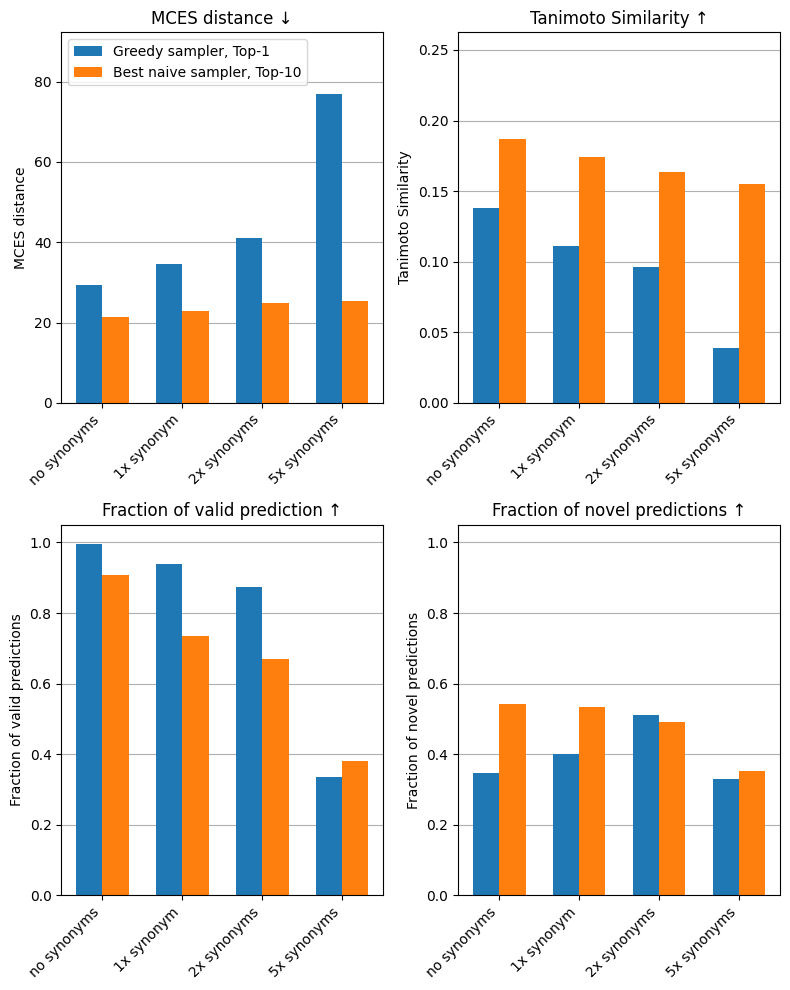
\includegraphics[width=0.79\textwidth]{figures/results/smiles_augmentation_with_tanimoto.png}
    \caption{Evaluation on the validation set of SMILES models trained with different SMILES augmented datasets.}
    \label{fig:smiles_augm}
\end{figure}

\newpage
Overall, MassSpecGym's de novo SMILES model does not seem to benefit from any SMILES augmented data.
A possible explanation for this worse performance is that the SMILES generation algorithm by RDkit (without random graph traversal) is deterministic.
It uses a canonicalization algorithm to generate this deterministic SMILES-string \cite{daylight_smiles_theory}.
Even though multiple SMILES can map to the same molecular structure, this algorithm will always be able to generate the same canonicalized SMILES-string from a molecular graph.
All SMILES labels in the MassSpecGym use this canonicalized format. 
By making the SMILES generation random, it could make training harder for the model.

\subsection{Spectral augmentation}

Input spectra can be augmented by simulating variations in neutral losses through spectral shifts.
Labeled spectra were augmented by applying the same random mz-shift to the peaks of a spectrum and copying its SMILES label.
Two models were trained for this experiments, with $20\%$ and $100\%$ of the training spectra augmented (referred to as $20\%$ mz shift augm. and $100\%$ mz shift augm., respectively, in the results).
Again, the original training data is kept in the training set.
Figure \ref{fig:spectral_augm} shows the evaluated results of these models using different metrics and evaluation settings.
As usual, the full naive samplers top-10 temperature search results can be found in the Appendix Figure \ref{fig:spectral_augmentation_appendix}.

\begin{figure}[h]
    \centering
    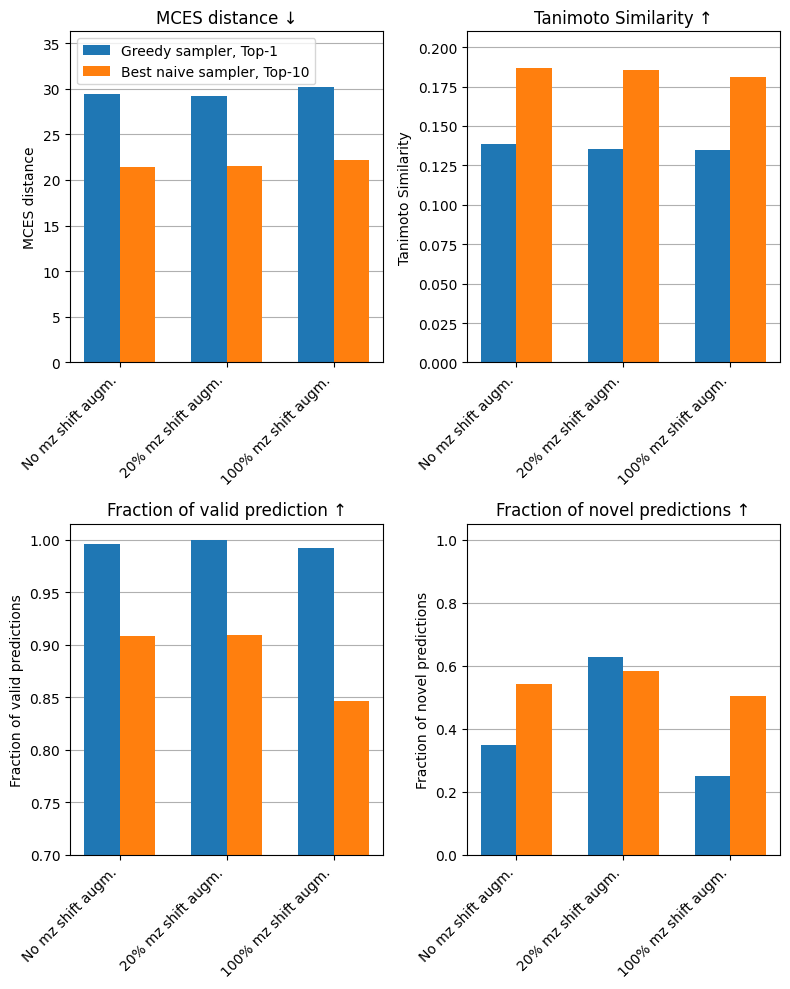
\includegraphics[width=0.7\textwidth]{figures/results/spectrum_augmentation_with_tanimoto.png}
    \caption{Evaluation on the validation set of SMILES models trained with different spectral augmented datasets.}
    \label{fig:spectral_augm}
\end{figure}

In contrast to the previous augmentation method, spectral augmentation does seem to help the de novo SMILES model from MassSpecGym.
While there are no considerable improvements looking at the MCES distance and Tanimoto similarity, the $20\%$ augmented model is able to predict more valid and especially more novel molecules.
Too much augmentation, again, hinders performance as the original data gets drowned in augmented data.

This method of augmentation, when moderately used, clearly seems to help the model be less prone to overfitting, as the top-1 greedy sampler is able to predict more than $20\%$ more novel molecules. 
However, to start from the same baseline, no augmentation is used in the next experiment.

\section{Molecular representations benchmark}

Different molecular representations can be used to predict the structure of a molecule.
This experiment benchmarks the string-based molecular representations from Section \ref{sec:molrepr} for the de novo structure prediction from \ac{MS/MS} task.
InchIkey is the only representation discussed in Section \ref{sec:molrepr} that is not used to train a model, as predicting hash keys is not possible.
All models were trained with the same hyperparameters.
Because tokenizers with a byte-pair encoded vocabulary have shown to influence performance, for each molecular representation, two models were trained.
One model used a byte-pair encoded tokenizer, the other used a basic character tokenizer.
This way, the influence of pretraining with \ac{BPE} can be measured for different molecular representations.
For all these models, a greedy sampler was used to evaluate the top-1 setting, while a temperature search was performed for the naive sampler with top-10 evaluation.
This ensures that the model is sampled in a exploitative and explorative setting.
Each molecular representation was thus evaluated four times.

\begin{figure}[h]
    \centering
    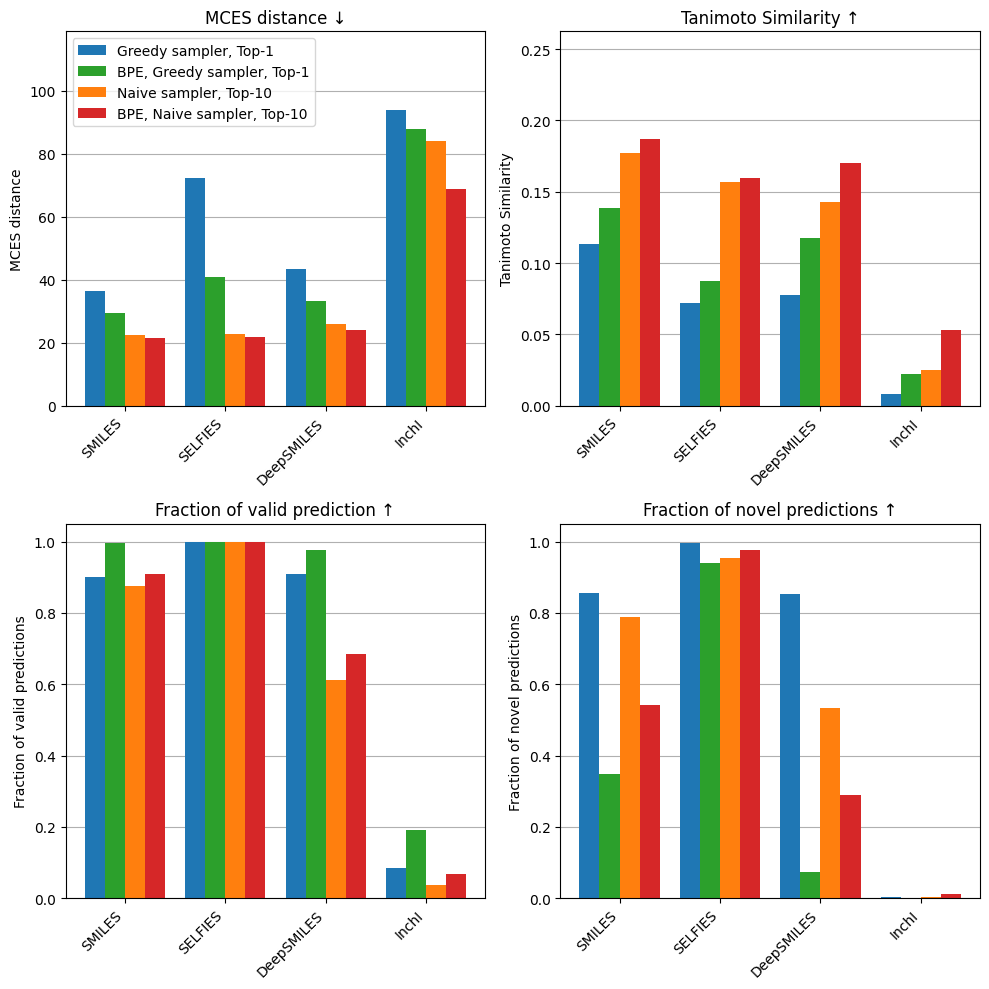
\includegraphics[width=0.8\textwidth]{figures/results/representations_with_tanimoto.png}
    \caption{Evaluation on the validation set of models trained with different molecular representations.}
    \label{fig:representations}
\end{figure}

The full results for the naive top-10 evaluation with different temperatures can be found in Figure \ref{fig:representations_appendix}.
Figure \ref{fig:representations} shows the MCES distance, Tanimoto similarity, fraction of valid predictions and fraction of novel predictions of the predictions from models trained on different molecular representations.

For the top-1 evaluation setting, SMILES outperforms the other molecular representations according to the MCES distance and Tanimoto similarity seen in Figure \ref{fig:representations}.
SMILES and SELFIES seem to perform the best for the top-10 evaluation according to their MCES distances, the Tanimoto similarity does not reflect this however, with the SMILES models outperforming the SELFIES models.

The models trained with SELFIES predicted the most valid predictions, as this is an inherent property of SELFIES, but noticeably also predicted the most novel molecules.
This indicates that the SELFIES models are less prone to overfitting on the training labels.

While DeepSMILES is closely related to SMILES with only slight modifications to reduce the chance of invalid predictions through syntax errors, it noticeably performs worse than SMILES, even having noticeably less valid predictions with top-10 evaluation.
The models trained using DeepSMILES are thus more prone to chemical errors as (almost) no syntax errors are possible.
An example of a prediction with a chemical error made by a DeepSMILES model can be seen in Figure \ref{fig:invalid_pred}, where five bonds on one carbon atom are present, which is not possible in a stable environment.
The improvements DeepSMILES introduces over SMILES to combat invalid predictions for autoregressive generation seem to have the opposite results for de novo structure prediction, by introducing more chemical errors.
\begin{figure}[h]
    \centering
    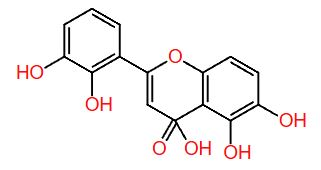
\includegraphics[width=0.5\textwidth]{figures/results/invalid_pred.JPG}
    \caption{2-dimensional representation of prediction with chemical error. (SMILES: C1=CC=C(C(=C1C2=CC(=O)(C3=C(O2)C=CC(=C3O)O)O)O)O )}
    \label{fig:invalid_pred}
\end{figure}

Out of the four representations benchmarked, InchI clearly shows to be the least fit for autoregressive generation, with most of its predictions being invalid.
This is caused by the fact that InchI has a strict layered structure to ensure its desired properties, which the models struggle to predict correctly.
When the model does succeed to predict an InchI with a valid syntax, it almost always was present in the training set, showing heavy signs of overfitting.
To help the model understand the different layers of the InchI representation, a separate model was trained with a different decoder for each relevant InchI layer. 
The results for this model can be found in Figure \ref{fig:layered_inchi}.
Unfortunately, while the decoders did achieve at predicting valid predictions for their corresponding layer, the strict InchI structure needed them to exactly describe the same prediction.
This model was only able to predict a few valid predictions and struggled to synchronize the outputs of the different decoders.
A possible improvement for this model would be to add a way to pass attention between the different decoders, these decoders could then synchronize their predictions to the same molecular structure.
The poor performance of InchI for this task is expected, as the molecular representation was not designed for structure prediction.

The same conclusions from the \ac{BPE} experiment can be drawn for this experiment, where the use of a pre-computed vocabulary using \ac{BPE} improves the MCES distance and number of valid predictions, but makes the model more prone to overfitting by having less novel predictions.
SELFIES is the only molecular representation from the benchmark where the number of novel predictions does not substantially drop when using \ac{BPE}.
This could be explained by the fact that some SELFIES tokens can have a different meaning in context of rings and branches. 
For example, a token that follows a branch token only denotes the length of the branch, the original chemical meaning of the token does not matter for the prediction.
When this combination of branch and other token is stored with \ac{BPE}, the model cannot get confused by the original meaning of the second token.
The SELFIES alphabet is also much larger than the SMILES alphabet, which causes the sequence of tokens to be more diverse, reducing overfitting.
Because each SELFIES stores a lot of information, fewer tokens are needed to describe molecular structures, which remarkably does not seem to affect the number of novel predictions.

Overall, in this experiment, SMILES shows to be the best molecular representation when a top-1 evaluation is used.
Taking the amount of novel predictions into account, SELFIES could also be considered for top-10 evaluation, as it shows to be much more robust against overfitting.

\chapter{Discussion}
\label{chap:discussion}

Intro discussion ? Poor performance?

\section{overfitting}

A recurring problem for the models trained for this thesis is the number of predictions that are identical to a label found in the training set.
When this occurs, it shows that a model is not able to achieve the task of predicting a de novo molecular representation from \ac{MS/MS}, but only repeats the data is has been trained with.
There are a few contributing factors to this overfitting problem with the setup used in this thesis.

\begin{description}
    \item[Duplicate training labels]
            As mentioned in the paper from MassSpecGym \cite{bushuiev2024massspecgym}, the dataset is a collection of the most qualitative annotated open-source mass spectrometry datasets.
            Even though a lot of filtering was performed after thorough quality control, the amount of duplicate molecules is significant.
            Figure \ref{fig:duplicate_smiles} shows the amount of SMILES that have multiple occurrences in the training set. Notice the logarithmic y-axis for readability.
            Even though 84\% of unique molecules have 10 occurrences or less, some molecules are noticeably more present in the training set, with one molecule being present 477 times in the training set.
            This imbalance does not necessarily reflect the real-world imbalance of molecules as it is caused by the use of imbalanced datasets.
            This causes the models to be trained with a bias towards these more frequent occurring molecules in the training set.
            This imbalance is also present in the validation (and test) set, where the most frequently occurring molecule accounts for 2.7\% (out of the almost 20.000 entries) of the validation data.
            Because of this imbalance, the models will be evaluated with a bias towards these more abundant molecules.
    \begin{figure}[h]
        \centering
        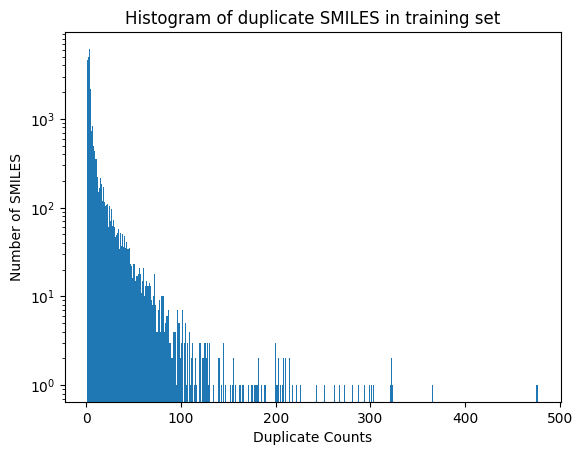
\includegraphics[width=0.6\textwidth]{figures/discussion/duplicate_smiles_training_set.png}
        \caption{distribution of duplicate SMILES in MassSpecGym's training set with a logarithmic scale}.
        \label{fig:duplicate_smiles}
    \end{figure}

    \item[Exposure bias] During training, a teacher forcing approach is used, where only the ground truth tokens are used to generate the next token iteratively.
    At inference time, when the model is sampled, the model does not get this help and has to rely on its own previous (incorrect) predictions.
    This is often referred to as exposure bias \cite{schmidt2019generalization}.
    The previously discussed imbalance of the training set only makes this bias worse, by training on these frequently occurring token combinations.
    This severely hinders the generalization of the model.
    An example of this exposure bias can be clearly seen in the results from the hyperparameter gridsearch (figure \ref{fig:gridsearch_vs_paper}), where a model with a lower validation loss performed worse at inference time.
    The loss has this teacher forced advantage, while the metrics calculated on the sampled predictions do not.
    Because all models trained in this thesis are optimized for validation loss, it can be questioned if they have been overfit on these teacher forced predictions.
    
    \item[MCES distance] Does not show overfitting 
\end{description}






%\section{Retraining MassSpecGym}
- loss function not optimal to determine model performance
- The SMILES validity is something the loss function can not measure.

overfitting:
    - dataset labels unbalanced
    - MCES distance does not show overfitting
    - teacher forcing + loss does not allow the model to predict synonym smiles




\section{Experiments}

SMILES veel overfitting, invloed op experimenten?

\subsection{Samplers benchmark}

- Beam search: Score function using loss is not optimal
\subsection{\ac{BPE} as pretraining}


\subsection{Augmentation}
Only BPE encoded SMILES models, overfitting might influence results

\subsection{SMILES augmentation}
- SMILES from molecular graph is deterministic, evaluation is done on only these deterministic outputs, by randomizing the SMILES with synonyms it confuses the model and will perform worse on the evaluated SMILES.
- model not powerfull enough
- BPE does not help because augmented patterns use more tokens
- less augmentation

\subsection{Spectral augmentation}

Could be used to fix mulecule imbalance, where only the least occurring molecules in the training set are augmented


\subsection{Molecular representations benchmark}

Models not optimized for hyperparameters
samplers chosen based of SMILES results

3 headed inchi could be improved by supplying the output of the previous decoder to the next, to ensure they know what molecule it is trying to predict

SELFIES can benefit from BPE because some tokens have different meaning in context of rings and groups, without the model overfitting

\section{Future for de novo structure prediction}

- string based representations not suited, reference graph based paper
- autoregressive models not suited for molecular structure generation by exposure bias
\input{chapters/methods}


% \input{Abstract}
% \input{Introduction}
% \input{Related_work}
% \input{Aims}
% \input{Results}
% \chapter{Methods and Materials}
\label{chap:methods}

All code used for this thesis can be found on \url{https://github.com/wwelvaer/thesis/tree/main/MassSpecGym}

\section{Model Training}
\label{sec:training}

All models trained for this thesis use the dataset described in section \ref{subsec:massspecgymdataset} and follow the de novo model architecture from MassSpecGym~\cite{bushuiev2024massspecgym} closely.
Most of the model architecture code was heavily inspired by MassSpecGym's source code.
It uses the pytorch transformer implementation along with a linear layer before and after the transformer to achieve the requested input and output dimensions.
The training algorithm follows the original transformer implementation from \textcite{vaswani2017attention}.
The result is a model that predicts the probability distribution of the next token given the peaks of a \ac{MS/MS} spectrum along with an already generated context sequence of tokens.

The exact model used in MassSpecGym suffered from exploding gradients in the first linear layer, which caused the computation to halt by overflow errors.
Several solutions were implemented to combat this problem.

\begin{description}
    \item[Gradient clipping]limits the gradient to an interval (often [-1, 1]),
    when during backpropagation a gradient is not in the interval,
    it is clipped to the closest boundary.
    \item[Lowering learning rate]of the affected layer delays the gradients from overflowing.
    \item[Scaling]the m/z values down to the same interval as the intensities.
    \item[Lowering the floating point precision]by shortening the mantissa to 7 bits instead of 23 bits (see figure~\ref{fig:bf16}), 
    all values get rounded to a lower precision. This rounding acts as a regularization step.
    \begin{figure}[h]
        \centering
        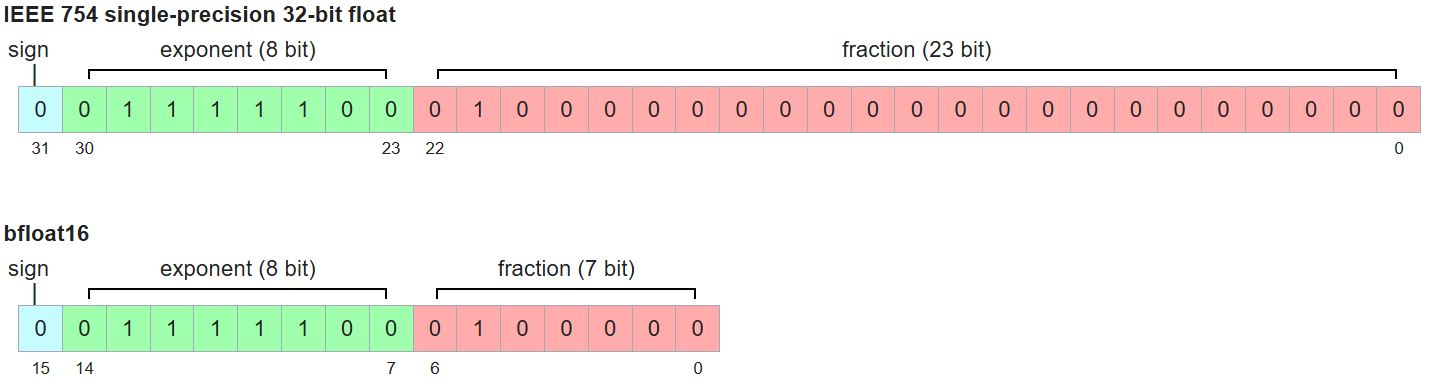
\includegraphics[width=\linewidth]{figures/methods/bf16.JPG}
        \caption{Composition of float32 and bfloat16}
        \label{fig:bf16}
    \end{figure}
    \item[Removing embedding scaling,]because the order of the peaks from the input spectra does not matter,
    no positional encodings are added, there is therefor also no need to scale the embedding layer as in the original implementation from \textcite{vaswani2017attention}.
\end{description}

Removing the embedding scaling was the only method that fully stabilized the training without tanking the performance.
All models described further therefore share the same model architecture as the MassSpecGym de novo models without the embedding scaling step.

All models were trained on the Ugent HPC accelgor cluster using a singular NVIDIA Ampere A100 GPU.
Training time without sampling was for every model around 2 hours. 

% Verplaatsen naar results?
To replicate the results from MassSpecGym, a hyperparameter gridsearch was conducted taking the optimal hyperparameters (= hyperparameters from the model with the lowest validation loss) from the MassSpecGym results into account
while also extending the search space further than the previously found optimal values.

\begin{table}[h]
	\caption{
		Gridsearch MassSpecGym vs Gridsearch from this Thesis (lowest validation loss models in bold)
	}
    \resizebox{\textwidth}{!}{
	\begin{tabular}{p{6cm}W{c}{4cm}W{c}{4cm}}
		\toprule
                \textbf{Hyperparams} & \textbf{MassSpecGym} & \textbf{Thesis Gridsearch} \\
            \midrule
                Learning Rate & $\mathbf{3\cdot 10^{-4}}, 1\cdot 10^{-4}, 5\cdot 10^{-5}$ & $1\cdot 10^{-3}, 3\cdot 10^{-4}, \mathbf{1\cdot 10^{-4}}$\\
                Batch Size & $512, \mathbf{1024}$ & $\mathbf{512}, 1024, 2048$ \\
                $k$ predictions & $\mathbf{10}$ & $\mathbf{10}$ \\
                Transformer hidden dimensionality & $\mathbf{256}, 512$ & $\mathbf{128}, 256, 512$ \\
                Number of attention heads & $\mathbf{4}, 8$ & $2, 4, \mathbf{8}$ \\
                Number of encoding layers & $\mathbf{3}, 6$ & $\mathbf{2}, 3, 4$ \\
                Number of decoding layers & $\mathbf{4}$ & $2, 3, \mathbf{4}$ \\
		\midrule
	\end{tabular}}
	\label{tab:gridsearch}
\end{table}

%%

\section{Samplers}
\label{sec:samplers}

\section{Augmentation}
\label{sec:augmentation}

\section{Molecular representations}
\label{sec:representations}

% \input{Discussion}

\printbibliography

\appendix
\chapter{Appendix}
\label{chap:appendix}

A few experiments / results that are not that relevant for the scope of this thesis are mentioned in this section.

\section{Sampler parallelization}
\label{sec:sampler_parallelization}
Figure \ref{fig:sampler_parallelization} shows the benchmark results between the naive sampler with and without parallelization.
The benchmark was performed on a singular NVIDIA Ampere A100 GPU.
\begin{figure}[h]
    \centering
    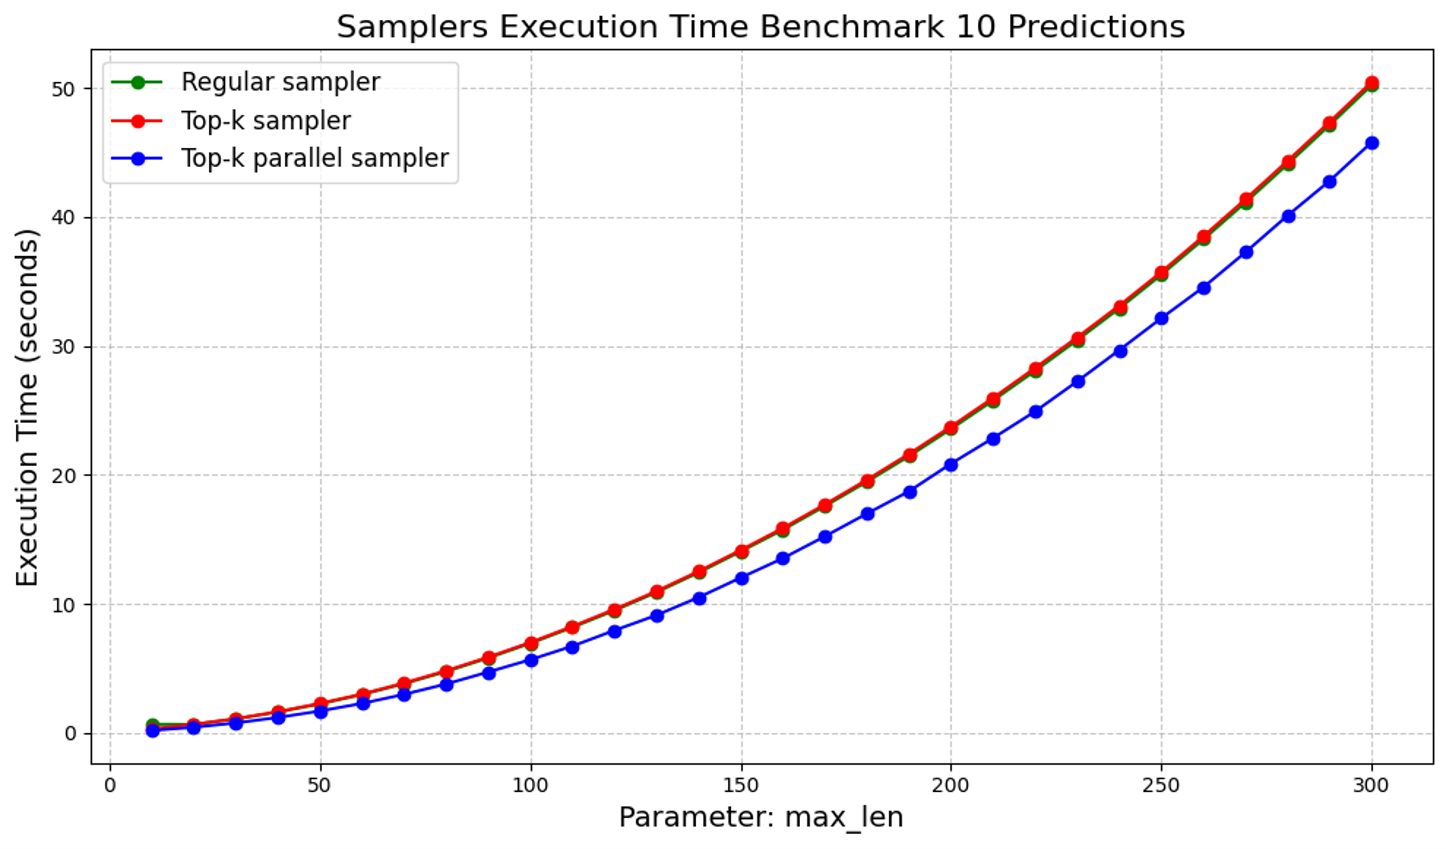
\includegraphics[width=0.6\linewidth]{figures/appendix/sampler_parallel.png}
    \caption{Execution Time Benchmark sampler parallelization}
    \label{fig:sampler_parallelization}
\end{figure}

The naive sampler shows to be more computationally efficient with parallelization.
A small difference in execution time can be substantial when this sampler is called thousands of times.
All further stochastic samplers in this thesis were executed with this parallelization enabled.

\section{Stochastic samplers benchmark full results}
\label{sec:sampler_full_results}

Figures \ref{fig:top-k_appendix}, \ref{fig:top-k_zoomed_appendix}, \ref{fig:top-p_appendix}, \ref{fig:top-p_zoomed_appendix} show the full results from the top-k and top-p benchmark.

\begin{figure}[h]
    \centering
    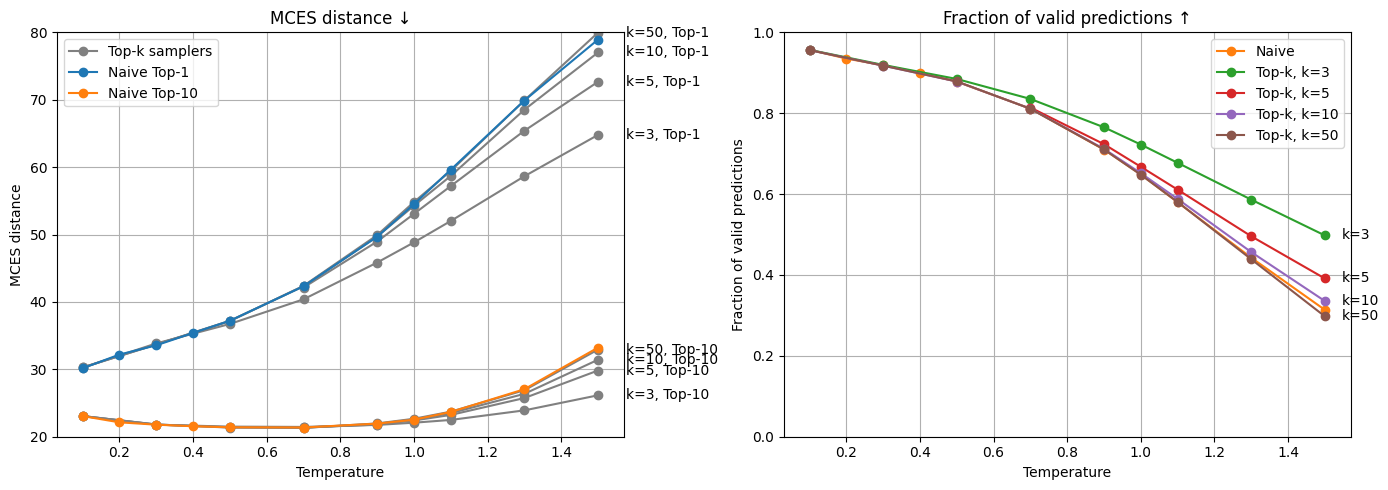
\includegraphics[width=\linewidth]{figures/appendix/samplers/top-k_vs_naive.png}
    \caption{Full top-k benchmark with top-1 and temperature search results}
    \label{fig:top-k_appendix}
\end{figure}

Top-k with $k=20$ is left out of figure \ref{fig:top-k_appendix} for readability. These results are in line with the others.

\begin{figure}[h]
    \centering
    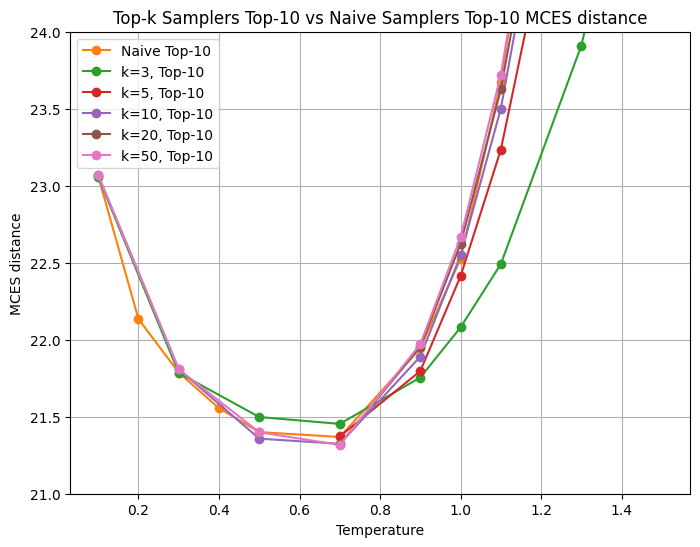
\includegraphics[width=0.6\linewidth]{figures/appendix/samplers/top-k_vs_naive_top-10.png}
    \caption{Zoomed in top-k top-10 MCES distance}
    \label{fig:top-k_zoomed_appendix}
\end{figure}

Figure \ref{fig:top-k_zoomed_appendix} shows the slight improvement of top-k $k\geq 10$ to the naive sampler in the temperature optima.

\begin{figure}[h]
    \centering
    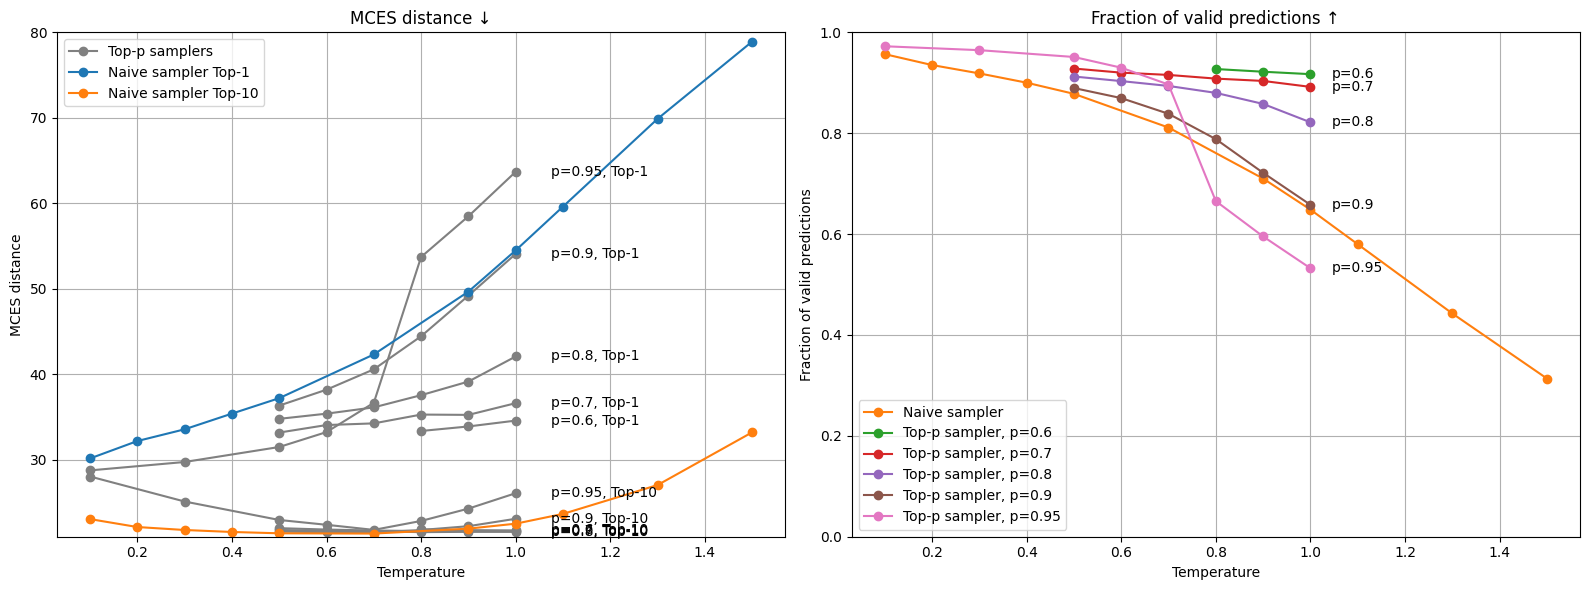
\includegraphics[width=\linewidth]{figures/appendix/samplers/top-p_vs_naive.png}
    \caption{Full top-p benchmark with top-1 and temperature search results}
    \label{fig:top-p_appendix}
\end{figure}

The search grid for the top-p benchmark was for some values of $p$ cut short to save resources.

\begin{figure}[h]
    \centering
    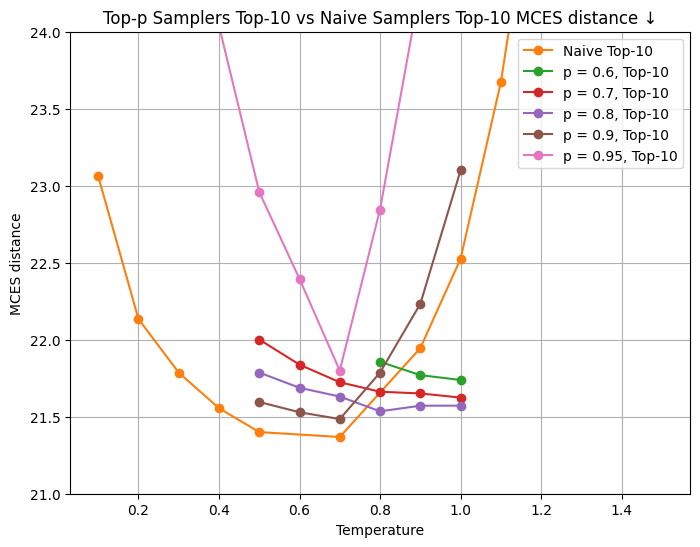
\includegraphics[width=0.6\linewidth]{figures/appendix/samplers/top-p_vs_naive_top-10.png}
    \caption{Zoomed in top-p top-10 MCES distance}
    \label{fig:top-p_zoomed_appendix}
\end{figure}

Figure \ref{fig:top-p_zoomed_appendix} shows that the top-p sampler results do not exceed the results from the naive sampler in their temperature optima.


\section{Top-10 Naive sampler temperature search results}
\label{sec:temp_search_appendix}

\begin{figure}[h]
    \centering
    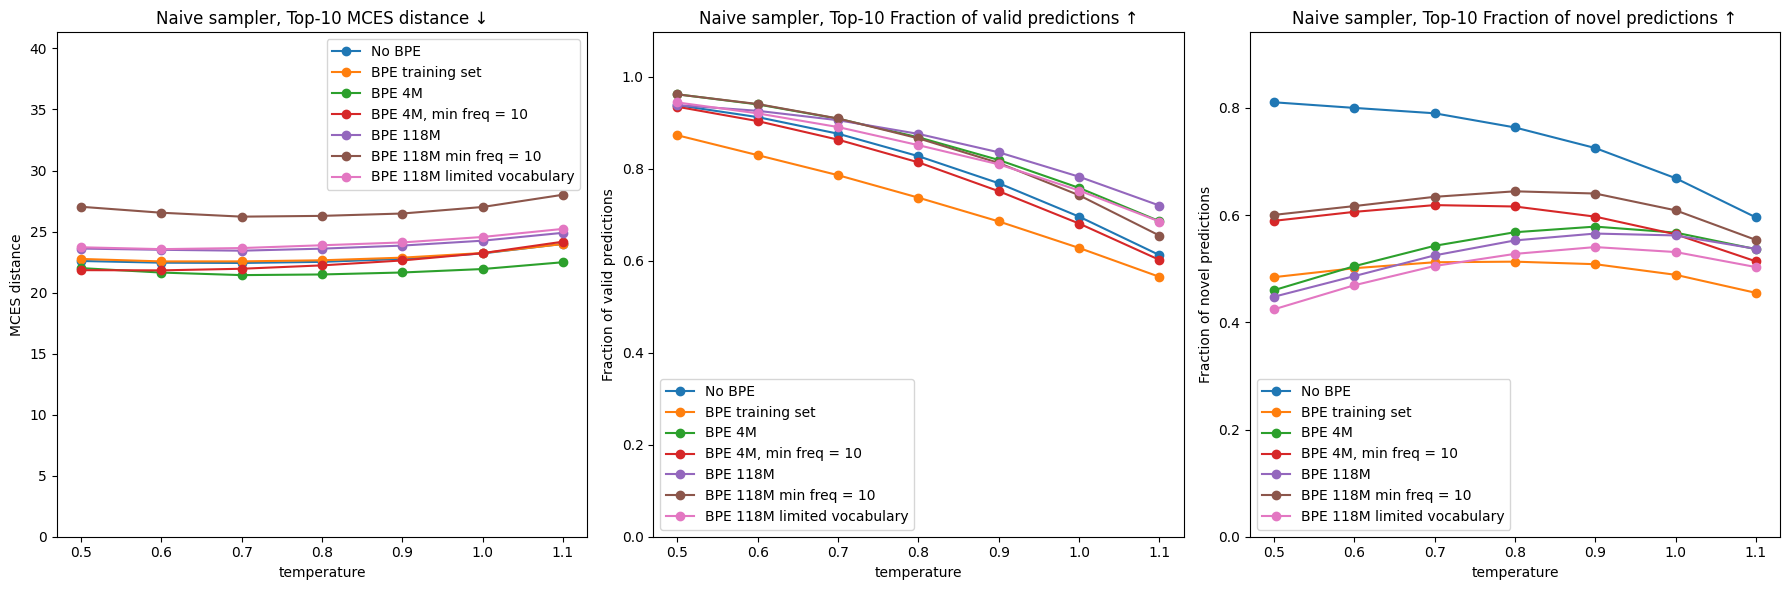
\includegraphics[width=1.0\textwidth]{figures/appendix/bpe.png}
    \caption{Top-10 Naive sampler temperature search BPE experiment results}
    \label{fig:bpe_appendix}
\end{figure}

\begin{figure}[h]
    \centering
    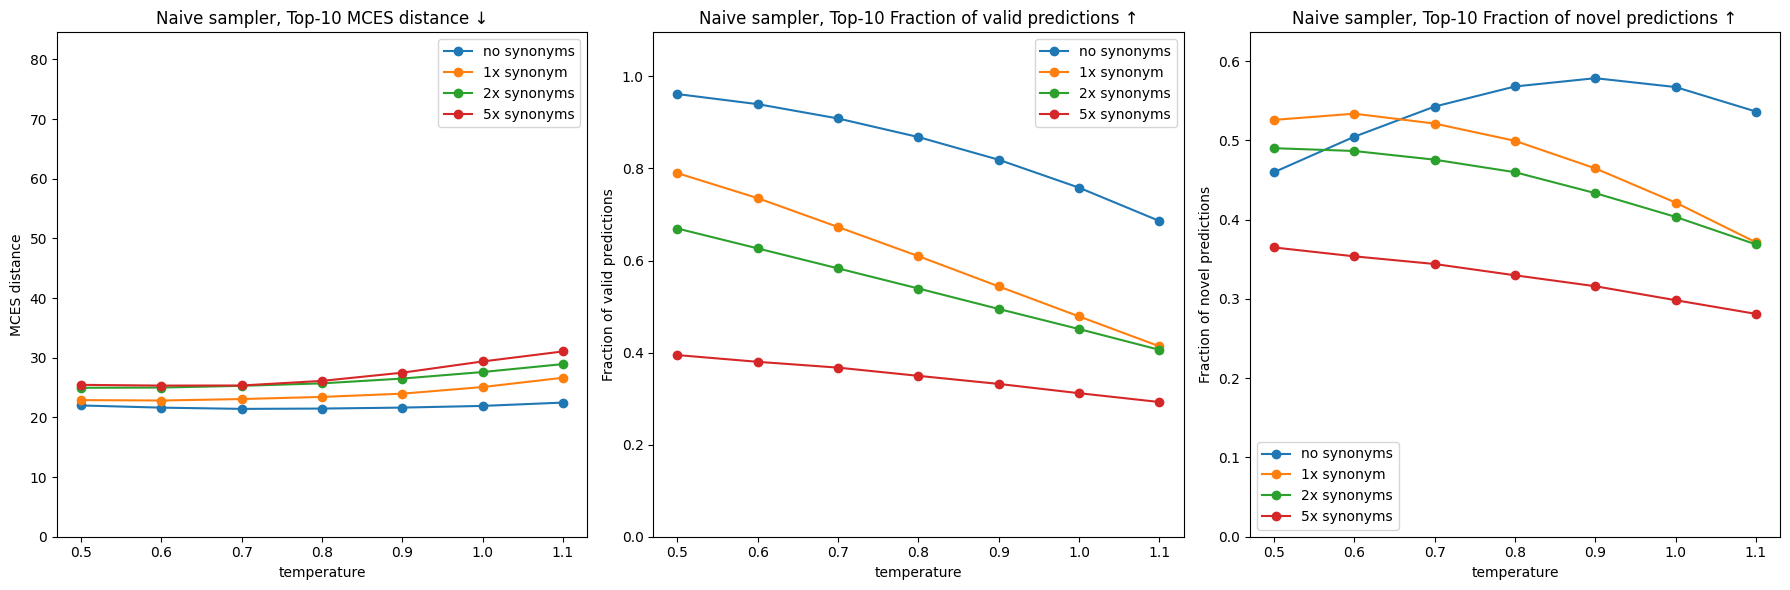
\includegraphics[width=1.0\textwidth]{figures/appendix/smiles_augmentation.png}
    \caption{Top-10 Naive sampler temperature search smiles augmentation experiment results}
    \label{fig:smiles_augmentation_appendix}
\end{figure}

\begin{figure}[h]
    \centering
    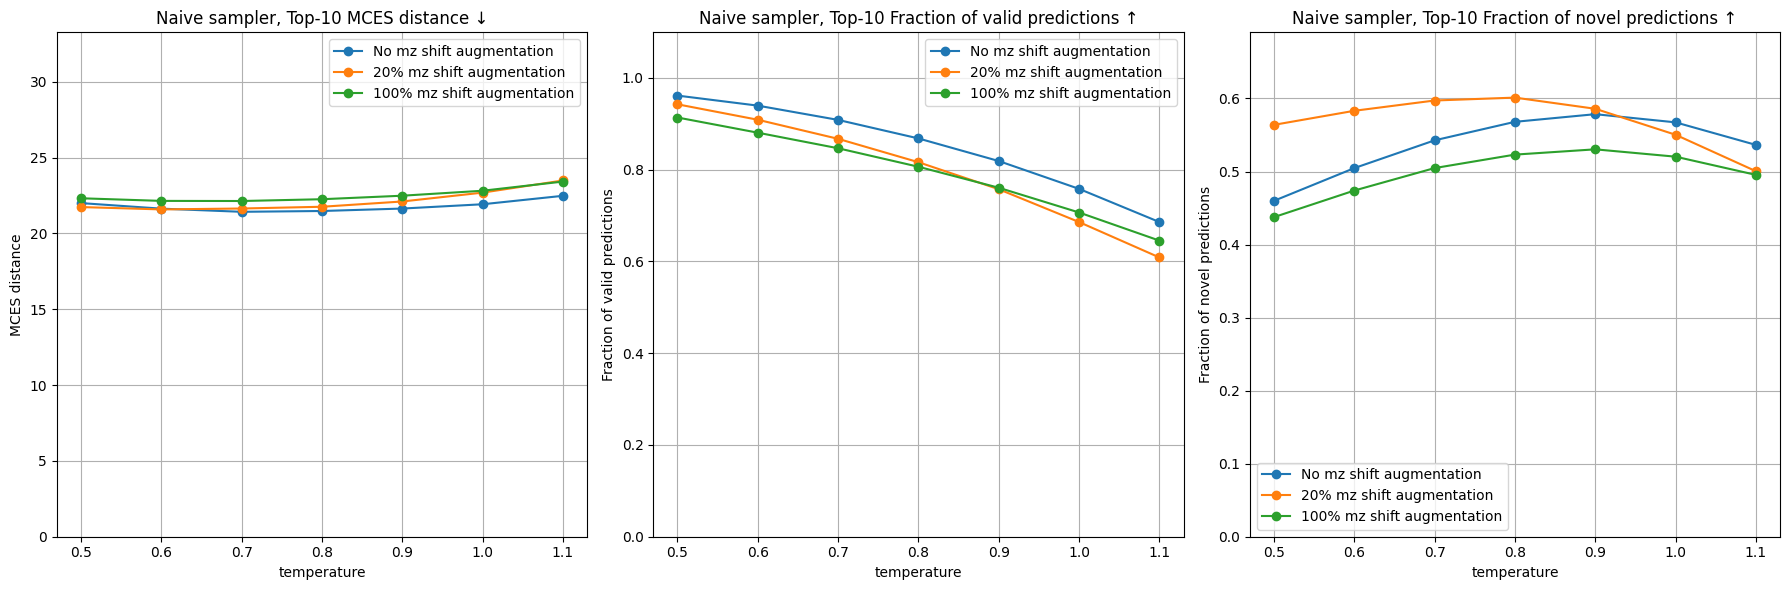
\includegraphics[width=1.0\textwidth]{figures/appendix/spectal_augmentation.png}
    \caption{Top-10 Naive sampler temperature search spectral augmentation experiment results}
    \label{fig:spectral_augmentation_appendix}
\end{figure}

\begin{figure}[h]
    \centering
    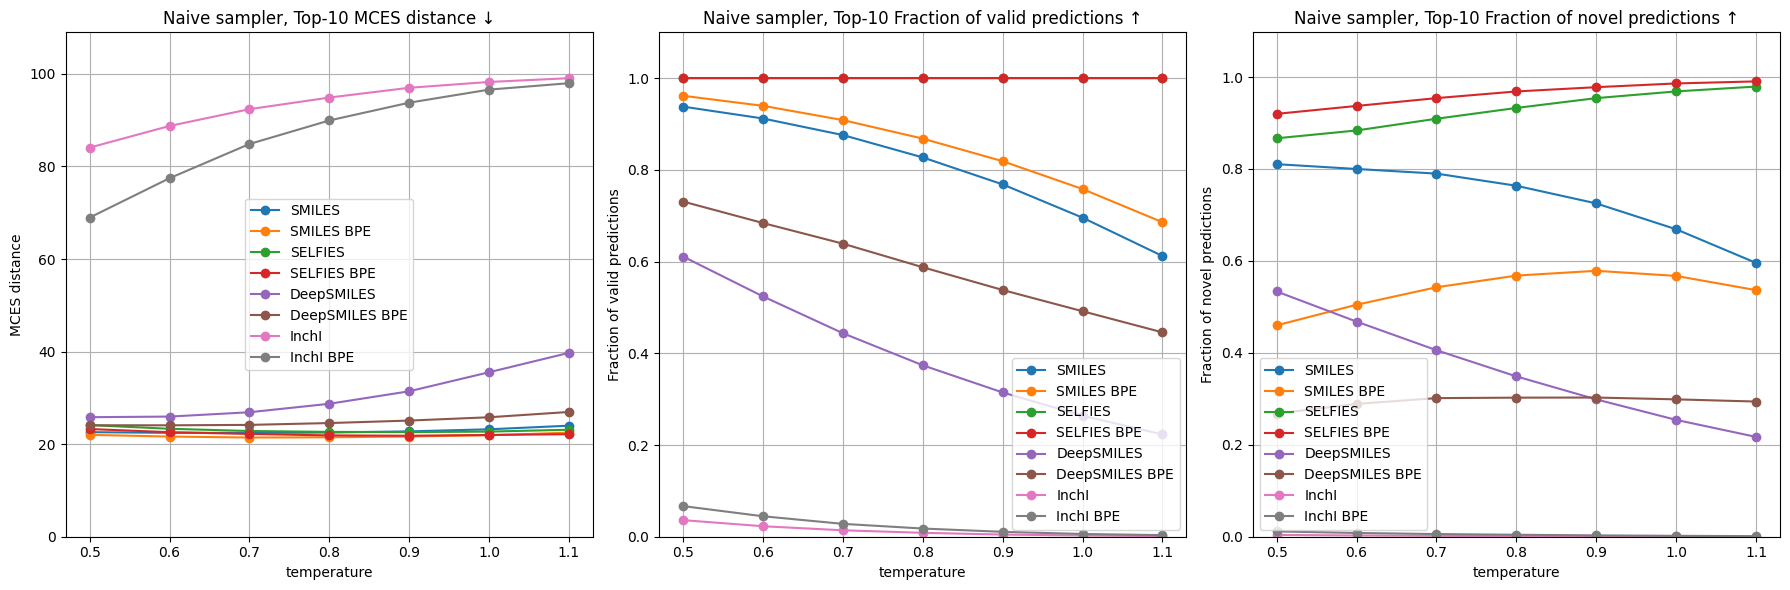
\includegraphics[width=1.0\textwidth]{figures/appendix/representations.png}
    \caption{Top-10 Naive sampler temperature search representations experiment results}
    \label{fig:representations_appendix}
\end{figure}

\begin{figure}[h]
    \centering
    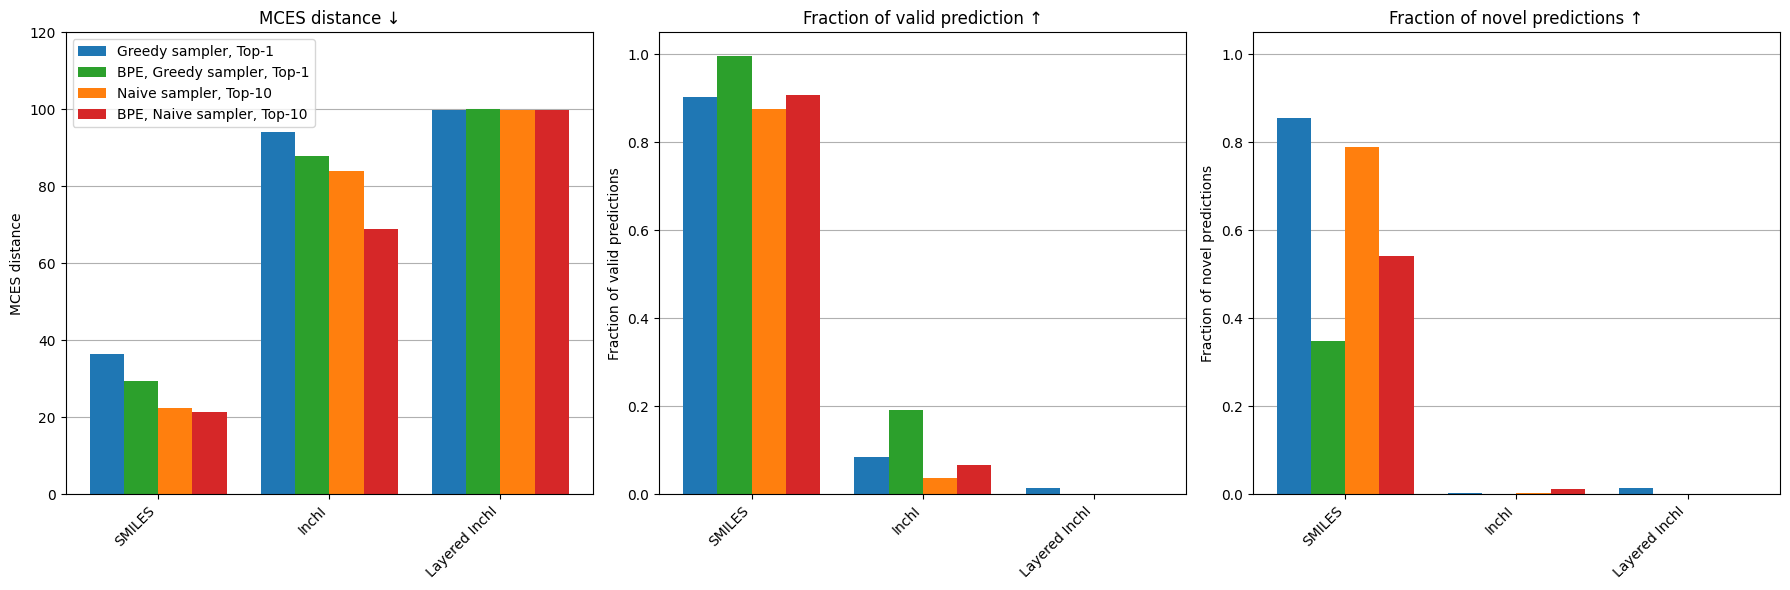
\includegraphics[width=1.0\textwidth]{figures/appendix/layered_inchi.png}
    \caption{}
    \label{fig:layered_inchi}
\end{figure}

% some empty pages
%\newpage\null\thispagestyle{empty}
%\newpage\null\thispagestyle{empty}
\end{document}
